\documentclass[11pt,,oneside]{fithesis}

\usepackage[english]{babel}
\usepackage[cp1250]{inputenc}
\usepackage[IL2]{fontenc}
\usepackage[plainpages=false, pdfpagelabels, hidelinks]{hyperref}
\usepackage{amsmath, amssymb, graphicx, amsthm, amsfonts, enumitem, algpseudocode, algorithmicx, wasysym, fixltx2e, float, etoolbox}

\setlist{noitemsep}

\usepackage{tikz}
\tikzset{ every node/.style={circle,fill=gray!15,draw,minimum size=1.5em,inner sep=2.5pt}}
\usepackage{array}

\usepackage[document]{algorithm}
\newfloat{algorithm}{t}{lop}
\floatname{algorithm}{Algorithm}
\renewcommand{\algorithmicrequire}{\textbf{Input:	}}
\renewcommand{\algorithmicensure}{\textbf{Output:	}}
\renewcommand{\algorithmicforall}{\textbf{for each}}
\let\ForEach\ForAll
\def\NoNumber#1{{\def\alglinenumber##1{}\State #1}\addtocounter{ALG@line}{-1}}

\newtheorem{thm}{Theorem}[section]
\newtheorem{lemma}[thm]{Lemma}
\newtheorem{proposition}[thm]{Proposition}
\newtheorem{corollary}[thm]{Corollary}
\newtheorem{definition}[thm]{Definition}
\AfterEndEnvironment{definition}{\noindent\ignorespaces}

\theoremstyle{definition}
\newtheorem{example}[thm]{Example}
\newtheorem{observation}[thm]{Observation}
\newtheorem{remark}[thm]{Remark}

\setcounter{figure}{0}
\makeatletter
\renewcommand{\thefigure}{\arabic{figure}}

\thesislang{en}
\thesistitle{Computational Complexity of Patrolling Games on Oriented Graphs}
\thesissubtitle{Diploma Thesis}
\thesisstudent{Mat�� Abaffy}
\thesiswoman{false}
\thesisfaculty{fi}
\thesisyear{2014}
\thesisadvisor{doc. RNDr. Tom� Br�zdil, Ph.D.}

\begin{document}

\FrontMatter
\ThesisTitlePage

\begin{ThesisDeclaration}
\DeclarationText
\AdvisorName
\end{ThesisDeclaration}

\begin{ThesisThanks}
I would like to thank Blablabla
\end{ThesisThanks}

\begin{ThesisAbstract}
Blablabla
\end{ThesisAbstract}

\begin{ThesisKeyWords}
patrolling games, game theory, complexity, algorithm, oriented graphs, blablabla
\end{ThesisKeyWords}

\MainMatter
\tableofcontents
\pagestyle{plain}

%TODO male pismena v nazvoch/nadpisoch
%TODO pisat bodky/ciarky za rovnicami?
\chapter{Introduction}

Blablabla

%do not forget motivation!


\chapter{Preliminaries}
% TODO review after writing the sections
In order to better understand the nature of patrolling games, we first introduce the concept of game theory.
Later in this chapter, we introduce security games, a special type of which are patrolling games. We mention some real-world applications of these theoretical models.
After that, we give an overview of patrolling games. We provide some examples and motivation why to study this field. We familiarize the reader with the basic terminology used throughout this thesis. We describe some special properties of the model of patrolling games we chose to study and we discuss the reasons why we did so.
The last section of this chapter we dedicate to the pioneers who set important directions of research in the field of patrolling games.

\section{Introduction to Game Theory}
In this chapter, we present the basics of game theory. The definitions and content used here are inspired by \cite{fudenberg}, \cite{polak} and \cite{gameTheory}.

Game theory is a mathematical study of decision making. It studies games as well-defined mathematical objects.
A \emph{strategic form} (or simply a \emph{game}) is played between \emph{players} $P_1, \dots, P_n, n \geq 2$.
Each player $P_i$ has a non-empty set $S_i$ of \emph{pure strategies}. A strategy can be seen as an algorithm telling the player what to do throughout the game.
The outcome of the game is an element from the set
$\mathcal{S} = \prod_{i=1}^n S_i$
and is called a \emph{strategy profile}.
Each strategy profile represents some value for every player.
Therefore, every player $P_i$ has his own \emph{utility function} $U_i: \mathcal{S} \to \mathbb{R}$ which assigns \emph{payoffs} to strategy profiles.
The higher the player's payoff of a strategy profile, the better the profile for the player.
The above representation of a game is called normal form. The normal game is usually represented by a matrix and is mostly used when a strategy represents a single action.

The extensive form of a game is appropriate to formalize games with time sequencing of \emph{moves}.
Here, games are played on trees, where each node with its outgoing edges represents a point of choice for a player.
Examples of both normal- and extensive-form games can be found in \cite{gameTheory}.

A \emph{zero-sum} game is a game such that $\sum_{i=1}^n u_i(s) = 0$ for all $s \in \mathcal{S}$.
In a two-player zero-sum game, one player's gain is equal to his opponent's loss.
Non-zero sum games are reffered to as \emph{general-sum} games.

Of great importance is the concept of \emph{mixed strategies}.
A pure strategy is a strategy which determines the move a player will make for every possible situation that could occur.
A mixed strategy is a probability distribution
%TODO odkaz na probability distribution?
over pure strategies.
Using a mixed strategy allows a player to randomize.
This means a player can make different moves under the same game conditions.
As each pure strategy is also a mixed strategy, we will refer to mixed strategies just as \emph{strategies}.

A player's \emph{best response} is the strategy (or strategies) which yields him the greatest payoff given the other players' strategies.

When it comes to solving the game, some form of equilibrium strategy profile is in demand. The best known solution concept in game theory is \emph{Nash equilibrium} (NE) \cite{nash}, in which no player can gain anything by changing only his strategy. That is, each player's strategy is a best response to the other players' strategies.

Different solution concepts were designed for specific game models. We are specially interested in the Stackelberg model, which we describe in the next section.

\section{Security Games}

Security games are two-player games in which \emph{defender} allocates resources to guard targets against an \emph{attacker} (also called \emph{adversary} or \emph{intruder}), who aims to attack some target.\footnote{In the rest of the paper, we denote the defender with "she" and the attacker with "he".}
Players' utilities are determined by the attacked target and the position of defender's resources during the attack.
If the target is defended (attack is unsuccessful), defender's utility increases and attacker's utility decreases.
Although one player's gain means other player's loss, security games are non-zero sum games in general.

A simple example of a security game is a problem of protecting $n$ banks in a city by $k, k < n$ policemen. Attacker wants to rob some bank and his attack is successful if and only if he attacks a bank without a policeman. The defender's goal is to distribute the security forces in a way that minimizes the probability of a successful attack.

In security games, it is mostly assumed that the attacker can observe the defender's moves and learn the defender's strategy before attacking.\footnote{In many situations attacker's perfect knowledge about the defender's strategy is at least questionable. Security games in which the attacker has only limited knowledge about the defender's strategy are studied e.g. in \cite{limited1, limited2, limited3, limited4}.}
This leads to adopting the \emph{Stackelberg} model.
In a Stackelberg game, the \emph{leader} (defender) first commits to a strategy, and then the \emph{follower} (attacker) chooses when and where to attack.
The standard solution concept for Stackelberg games is \emph{strong Stackelberg equilibrium} (SSE, also called \emph{leader-follower equilibrium}), which gives the leader the maximum expected utility in the worst-case scenario.
A crucial assumption is that the follower has a perfect knowledge of the defender's strategy and plays a best response to maximize his expected utility.
One of the advantages of an SSE is that being a Stackelberg leader cannot hurt the defender \cite{convex, nashStack}. Furthermore, under certain natural assumptions about security games, any SSE is also an NE \cite{interchangability}.

\subsection{Secuirty Games in Real World}

The leader-follower Stackelberg game model is actually utilized in many real-world security situations.
We are aware of five applications based on this model which were already put into use in the United States. We present them in chronological order as they were deployed.

The first deployed decision-support application is the \emph{ARMOR} (Assistant for Randomized Monitoring over
Routes) security system \cite{armor}.
It has been deployed since August 2007 at the Los Angeles International Airport (LAX).
It is used for randomizing allocation of checkpoints on the roadways and assigning canine patrol routes within the terminals.

The second application, deployed by Federal Air Marshals Service (FAMS), is called \emph{IRIS} (Intelligent Randomization In Scheduling) \cite{iris}.
IRIS helps to create a flight coverage schedule for armed marshals who can defeat terrorist attacks.
Scheduling constraints in IRIS are much more complex than in ARMOR as the marshals are limited by their location and timing constraints.
Although IRIS was developed for FAMS, it provides a general framework for solving patrolling scheduling problems in other transportation networks as well, e.g. in New York City subway system.

Another security application using the Stackelberg game model is the \emph{GUARDS} (Game theoretic Unpredictable and Randomly Deployed Security) system \cite{guards}.
It helps United States Transportation Security Administration (TSA) in resource allocation tasks for protection of more than 400 airports.
In constrast with ARMOR and IRIS, which focused on one security activity, GUARDS reasons about hundreds of heterogenous defender activities, large number of diverse potential threads, and hundreds of potential end-users.

Other example of a game-theoretic security system is \emph{PROTECT} (Port Resilience Operational/Tactical Enforcement to Combat Terrorism) \cite{protect}.
It has been currently deployed by the United States Coast Guard (USCG) in the ports of Boston, New York and Los Angeles \cite{protect_coastguard}.
In contrast to the three beforementioned security applications, PROTECT relies on a quantal responce (QR) \cite{quantal} model of the adversary's behavior, i.e. the attacker has only bounded rationality.
It was the first time that the QR model has been used in a real-world security application \cite{protect}.

The last real-world security application we mention is \emph{TRUSTS} (Tactical Randomization for Urban Security in Transit Systems) \cite{trusts}, used by the Los Angeles County Sheriff's Department (LASD).
The main purpose of TRUSTS is fare-evasion deterrence in urban proof-of-payment transit systems.
In these systems, passengers are legally, but not physically, required to purchase tickets.
Patrol units move about the system and fine fare-evading passangers.
The optimization objective is to maximize the total revenue (ticket sales plus fines) to the government.
In \cite{trusts2}, the authors extend the TRUSTS system to incorporate also crime prevention and counter-terrorism.

\section{Introduction to Patrolling Games}
\label{sec:PG}

In this section, we introduce the concept of patrolling games in general and we give a simplified motivational example of what it might look like in real life.
Later, we informally describe the model adopted by us and we discuss its advantages.

Patrolling games are a special type of security games.
Their unique feature is that the defender's resources can change their position in time.
Furthermore, the attacker needs some finite time, called \emph{penetration time} (also \emph{attack length}), to succesfully complete an attack on a target.
During this time, the defender can detect the intrusion in which case the attack is unsuccessful.
The defender's goal is to commit to a strategy which maximizes the probability of detecting an intrusion.
The attacker's goal is to maximize the probability of a successful attack.
The resources controlled by the defender are called \emph{patrollers} (also \emph{robots}).
As the defender is represented by her resources, we use these two terms interchangably.
That is, under "defender" we might mean her resources and vice versa.

We illustrate the problem of patrolling on a simple example mentioned in \cite{miso}.
Let us assume a city with $n$ banks which the police can protect against robbery.
The police have $k, k < n$ police officers with cars available.
We assume that banks cannot let the police know that an attack is under way.
The goal of the police is to create a surveillance plan which minimizes the possilibity of a successful attack.

\

There are many models of patrolling games which differentiate from each other in many ways (see Section \ref{sec:patrolLiterature}).
We work with a simple model of patrolling games which was introduced in \cite{miso}.
The results achieved in this thesis can be easily extended to more general models, which is explained later.
%TODO link where the explanation is

We model a patrolling game as a two-player zero-sum Stackelberg security game in extensive form with infinite horizon.
The game is played on a directed graph, which represents the possible locations and moves of the defender.
Some of the nodes of the graph are targets, all of which are equivalent:
the attacker and the defender have no preferences over the targets and the attacker needs $d \geq 1$ time units to successfully attack any target.
The defender starts in some initial target node and moves from node to node.
Every move, consisting of the defender traversing an arbitrary edge, takes one time unit (step).
The defender chooses the next node randomly and based on the history of all already visited nodes.

The assumed Stackelberg model implies a strong adversary, i.e. the attacker has complete knowledge of the defender's strategy and her current position.
As the attacker observers the defender, he may either wait, or attack some target.
When he attacks a target, he has to stay there for the next $d$ steps, i.e. he cannot leave even if he sees the defender approaching.
Realize that a strong adversary would never attack a target currently visited by the defender.
However, he can attack this target right after the defender's departure, long before the attacker arrives to the next node.
That leads us to the following definition of a detected attack---if the defender is in node $v$ and the attacker attacks a target $u$, the attack is detected and the attacker is captured if and only if the defender visits $u$ in the next $1, \dots, d$ steps, even if $u = v$ \cite{iti1}.
Otherwise, the attack is successfully completed.
We assume the game ends after the attack is detected or completed, i.e. no more than one attack is possible.
The defender aims to minimize the probability of a successful attack, the aim of the attacker is the opposite.

The Stackelberg setting enables the attacker to play the best response to the defender's strategy.
Therefore, the attacker cannot increase his utility using randomization, so we consider only pure attacker's strategies.
Note that we model a patrolling game as a zero-sum game, i.e. the higher the attacker's utility, the lower the defender's utility.
This means the attacker's best response represents the worst case for the defender.
In other words, the attacker tries to hurt the defender as much as possible.
Bear in mind that when finding the optimal strategy for the defender, we are concerned with the worst case scenario.

For now, we assume that the defender has only one patrolling unit as we draw on the results achieved in \cite{miso, iti1}.
We generalize this model by allowing multiple patrolling units in Chapter \ref{chap:multiPatrol}.

From now on we also assume a single adversary who can attack only with a single resource.
This assumption is adopted by all of the works mentioned in Section \ref{sec:patrolLiterature} as well.

The reasons for choosing this model are described in detail in \cite{miso}.
The basic motive is to consider a model as simple as possible, yet still reasonable enough.
This motive resulted in opting of the following parameters of our model: graph structure, discrete time, no preference over targets, unified attack length, immobile targets, and only one attack possible.

It turns out that the assumption of all edges being of length 1 is quite sufficient. Indeed, the case where edges can have different natural lengths can be reduced to our simple model by splitting each edge of length $t$ to $t$ sequentially connected edges of length one. A more general case with rational lengths of edges can be reduced to the previous case by multiplying both the lengths of edges and the attack length by a suitable number.

The motives behind choosing the Stackelberg model are not restricted to simplicity.
Besides the reasons mentioned in \cite{miso}, the Stackelberg setting together with the game being zero sum lead to one favorable characteristic---the optimal defender's strategy is optimal also with respect to the worst-case scenario.

The motive for absolute optimality led to allowing the defender to make her movement choice based on all the moves she already did.
This is in contrast with all the other patrolling literature we are aware of, where the defender can decide where to move based only on the last $h$ visited nodes.
Strategies with $h = 1$ are based only on the current defender's location and we call them \emph{stationary} (or \emph{Markovian}).
In \cite{arbitrary} there is an example where no optimal defender's strategy is stationary.
In \cite{iti2} it has been shown that, in general, there might be no optimal defender's strategy which depends only on the last $h$ visited nodes for any $h \in \mathbb{N}$.

%TODO \section{Related Work}
\section{Basic Literature on Patrolling Games}
\label{sec:patrolLiterature}
In this section, we give an overview of the research in the field of the patrolling games in the last years. We address several papers and models. For each paper, we state the differences from our model and we mention the most significant results achieved.

In the rest of this section, we use the following assumptions which hold true unless stated otherwise.
A patrolling game is played on a directed graph with distances between any two neighbour nodes being the same.
We assume a Stackelberg game model, i.e. the attacker knows the defender's strategy and the current position of the patrolling unit(s).
And to intercept an attack, the defender has to come to the node where the attack is taking place.

\subsection{Perimeter Patrol}
The first reference in almost every robot patrolling paper is \cite{perimeter}. The authors consider a problem of multi-robot patrol around a closed area with the existence of a single adversary trying to enter the area. A real life motivation might be the following scenario. An intruder tries to cross a border while some patrolling units aim to detect this intrusion.

The authors show that in adversial settings non-deterministic defender strategies are needed. They demonstrate it on an example similar to the following situation. A robot moving with velocity ${1m/s}$ is required to patrol around a fence of length 25 meters. Assume that an adversary needs 20 seconds to penetrate the area through the fence. If the robot moves deterministically, in any point of time a fence section of lenght of at least 5 meters will not be visited by the robot in the next 20 seconds. The intruder can guarantee penetration by entering through this section. However, if the robot moves in a non-deterministic way, it can commit to a strategy that does not allow the adversary to penetrate the area with probability 1.

In the paper, a circular graph is considered. All nodes of the graph are targets with unified attack length. A system consisting of $k$ mobile robots is considered. Robots move simultaneously. The model is Markovian, where for each node the robot goes to the right with probability $p$ and to the left with probability ${1 - p}$.\footnote{Two other movement models, where the robot has directionality associated with its movement, are considered. The achieved results, such as polynomial time algorithm for finding the optimal strategy, apply for these models too.} The authors prove that to maximize the probability of penetration detection (\textsf{ppd}), the robots have to be placed uniformly along the cycle and they have to be coordinated, i.e. all robots move together in the same direction. This reduces the problem to a much simpler instance with smaller graph and only one robot. The main result is a polynomial time algorithm which computes the optimal defender's strategy.

Authors' subsequent papers concerning multi-robot perimiter patrol in adversial settings include \cite{perimeter2} and \cite{perimeter3}. In \cite{perimeter2} it is shown that in the case the adversary has no knowledge of the patrol scheme, a deterministic algorithm is optimal. However, the deterministic algorithm creates high deviations between the  \textsf{ppd} values in the nodes and it is easy to detect. Therefore, the authors present an algorithm that deals with adversary having partial information. This algorithm maximizes the expected \textsf{ppd} along with minimizing the deviation between the \textsf{ppd} values throughout the perimeter. Its performance was verified by experiments with human subjects.

\subsection{Arbitrary Graph Topologies}

A more general graph topology is addressed in \cite{arbitrary}. The authors consider a model with a single robot patrolling on an arbitrary directed graph. Not all nodes of the graph are necessarily targets and each target node $i$ requires the intruder ${d_i}$ steps to enter.
The robot is equipped with a sensor able to detect the intruder. The robot's sensing capabilities are represented by a matrix ${V(n \times n)}$ where ${v_{i,j} = 1}$ iff node $j$ can be sensed from node $i$.
%TODO footnote?
The patroller's sensing capabilities in our model are equivalent to the case of $V$ being an identity matrix.

The possible outcomes of the game are defined as follows:
\emph{intruder-capture}, when the intruder attacks some node $i$ and the robot senses $i$ in the next ${d_i}$ steps;
\emph{penetration-i}, when the intruder attacks node $i$ and the robot does not sense $i$ in the next ${d_i}$ steps;
\emph{no-attack}, when the intruder never attacks.
For each possible outcome, patroller's and intruder's payoffs are defined.\footnote{The game is a general-sum game with some consistency constraints over the players' payoffs.} Explicitly, these values are known to both players. However, the model can capture the case when the intruder's preferences over the targets are uncertain to the patroller.

The authors cope with the presence of the infinite horizon in the game by introducing symmetries. They allow the patroller to choose the next action based only on the last ${|H|}$ actions, where ${|H|}$ is finite and constant during the whole game. Higher value of ${|H|}$ leads to possibly higher expected utility of the patroller, but also to higher computational complexity for finding the optimal patrolling strategy. The authors provide a multi-bilinear mathematical programming formulation to find the optimal patroller's strategy when ${|H| = 1}$. They state that formulations with ${|H| > 1}$ can be obtained by extending this one.

Further, the paper is concerned with heuristics for more efficient problem solving. In realistic settings, the number of targets is significantly smaller than the number of all nodes. That affords the opportunity to reduce the searching space, the number of variables and constraints, of the programming problems.
First, the authors are interested in a deterministic strategy which detects any attack with probability 1. To solve the problem of finding such a strategy, they formulate an integer linear program.
Second, the authors aim to minimize the number of nodes over which the patroller will randomize when using an optimal strategy. They formulate another integer linear program for that.
Third, they introduce the concept of action dominance for the intruder.
For an example setting, the reduction of nodes and the elimination of dominated actions resulted in the following improvement. Both the number of bilinear problems to be solved and the average computational time for solving a single problem decreased from ${29^2}$ to 18 and from more than 30 minutes to less than 5 minutes, respectively.

The rest of the paper discusses the problem of finding an upper bound for ${|H|}$, say ${|\overline{H}|}$, such that among all the strategies, there is an optimal strategy
which uses no more than length ${|\overline{H}|}$ of the history, i.e. for any ${|H| > |\overline{H}|}$ the patroller's expected utility keeps constant. Throughout the paper it is claimed that this treshold exists. However, in \cite{iti2} this claim has been proven \emph{incorrect}. Moreover, in \cite{arbitrary} they formulate a theorem that for a fully connected topology, ${|\overline{H}| = 0}$. That is also \emph{incorrect}. The proof sketch is done on a complete graph with 3 nodes, each with attack length 2. The authors prove that their algorithm gives the same expected utility when ${|H| = 0}$ and ${|H| = 1}$. Generalization of any kind is omitted. The highest expected utility when ${|H| = 0}$ is ${5/9}$. However, in \cite{iti1} there is a strategy with ${|H| = 2}$ giving expected utility ${(\sqrt{5} - 1)/2}$, which is strictly greater than ${5/9}$.

The authors extend the model from \cite{arbitrary} to more realistic settings in \cite{powerlessIntruder}. They weaken the intruder in two ways. Their first extension introduces the intruder's movement. The intruder does not appear directly at the target, rather he has to traverse the graph along paths connecting \emph{access areas} to targets. The intruder can move infinitely fast. Covering a path takes only one step during which the intruder can be detected on every node of the path. In their second extension, some cells are hidden to the intruder. As he cannot observe the whole environment, he cannot perfectly know the position of the patroller when attacking. A concept of a \emph{state} is introduced, representing when (how many steps ago) and where (in which node) has the patroller been observed for the last time. For both extensions the authors provide mathematical programming formulations, reduction algorithms and experimental evaluations.

\subsection{Multiple Patrolling Units}
\label{subsec:multi}

The authors of \cite{arbitrary} generalized their model by introducing multiple patrolling robots in \cite{multi-robot}. On the other hand, they simplified the model in many ways. They assume that the robots' strategy is Markovian, that the robots and the intruder have the same preference ordering over the targets and that the robots can sense only the nodes they are in.

%nejake odsadenie?
%podnadpis Smallest Number of Robots
The first problem addressed in the paper is finding the smallest number of robots needed to capture any attack with probability greater than zero. With a smaller number of robots the intruder could successfully attack with probability 1. The authors show that this problem is equivalent to finding the smallest number of maximal cliques such that each target belongs to at least one clique. A simplified idea behind this is the following.

Let us assume a setting with a graph $G$ and a set of targets $T$. Let $T' \subseteq T$ be a subset of targets. If there is a subgraph $G' \subseteq G$
%such that $T'$ is a subset of nodes of $G'$
%such that for each $t \in T'$ it holds that
%$t$ is a node of $G'$
such that for each $t \in T'$ and for each node $v$ from $G'$ there is a path from $v$ to $t$ in $G'$ of length at most $d_t$, then a single robot can patrol all the targets $T'$. In other words, the robot has a strategy such that in each node of $G'$, for all $t \in T'$ the robot will visit $t$ in at most $d_t$ steps with probability strictly greater than zero.
The goal is to find the smallest set of such subgraphs that would cover all the targets.

The authors build an abstraction $Q$ of the original graph $G$. They formulate an algorithm to find the set of all maximal \emph{labeled cliques} in $Q$
%these cliques represent the beforementioned subgraphs
and a linear program to find the smallest labeled clique cover. The result of the program is the smallest number of robots needed to patrol the environment.

%nejake odsadenie?
%podnadpis Coordination between Robots
The second problem studied in the paper regards the coordination between the robots. The authors consider two coordination dimensions, each with three possible values.

The first dimension refers to the degree of \emph{coordination in computing the patrolling strategy}, which can be of one of the following types: 

\emph{Joint strategy}: the strategy of each robot depends on its position and on the position of all the other robots.
One strategy regarding the movement of all the robots is computed centrally. The solution contains $O(n^{|R|})$ probability variables, where $n$ is the number of nodes and $|R|$ is the number of robots.

\emph{Disjointed strategies}: the strategy of each robot depends only on its position and contains information only about its movement. The strategy of each robot is computed centrally keeping into account the strategy of all the other robots. The solution contains $O(|R|\cdot n^2)$ probability variables.

\emph{Separated strategies}: each single robot computes its own strategy without considering the strategies or positions of the others. This reduces the multi-robot patrolling problem into a set of $|R|$ single-robot patrolling problems, each with $O(n^2)$ probability variables.

The second dimension refers to the degree of \emph{coordination in partitioning the environment}. Each robot is constrained to move within a portion of $G$ assigned to it. Possible levels of this coordination are:

\emph{Full assignment}: each robot can potentially move in every vertex of $G$.

\emph{Maximal clique assignment}: each robot is assinged a maximal labeled clique (in the abstraction $Q$ of $G$). If the cliques overlap, some targets may be patrolled by multiple robots.

\emph{Separated assignment}: as the previous case, but the cliques assigned to the robots may not overlap (they do not have to be maximal cliques). Therefore, each target is patrolled by only one robot.

In the next part of the paper, the authors combine the two mentioned coordination dimensions together. They show that only some combinations are reasonable. For example, joint strategy with separated assignment can be reduced to separated strategy with separated assignment. That is because robots patrolling separated portions of $G$ do not need to cooperate. A mathematical programming formulation is proposed for each reasonable combination of values.

Experimental results show that the higher the degree of coordination, the higher the computational effort and the robots' utilities.\footnote{There is an exception to this rule in the case of separated strategies: separated assignment turned out to be more time-consuming and gave higher utilities than maximal clique assignment. This shows that overlapping patrolling areas without any strategy coordination have negative effect on the expected utility.}
An easy observation was that joint strategies do not scale with large settings (more than 15 nodes) as they require much memory.
Special attention was paid to two coordination combinations: disjointed strategy with maximal clique assignment ($\mathcal{D}_3$) and separated strategy with separated assignment ($\mathcal{D}_5$). $\mathcal{D}_5$ consumed less time than $\mathcal{D}_3$ just because the number of possible assignments was small. With larger settings, the number of all the possible separated assignments increases drastically faster than the number of maximal cliques. Another interesting observation is that higher number of robots can lead to lower computational time. That is because adding more robots decreases the portion of $G$ assigned to each robot and the computational time strongly depends on the size of this portion. For~more~conclusions,~see~\cite{multi-robot}.

\subsection{Moving targets}

So far, the targets carrying value were static. In \cite{movingTargets}, the authors assume that these valuable targets can change their positions in time. This is motivated by real-world scenarios such as protection of vessels transiting waters with high pirate activity and unmanned aerial vehicle-based surveillance protecting moving ground targets.

The model considered in \cite{movingTargets} is based on the model used in \cite{arbitrary}. It assumes unified attack length and first-order Markovian defender's strategy.
In addition, targets are allowed to move through the area according to a deterministic movement schedule. This schedule is a fixed property of the environment and is known to both players.

The game is played in $|T|$ turns, thereafter it is repeated \--- i.e. the targets move in cycles. In each turn, the defender can move to an adjacent node and the targets can move to any node. The movement of the targets is defined by an arbitrary function ${f : Q \times T \to V}$, where $Q$ is the set of targets, $T$ is the set of turns and $V$ is the set of nodes.
%TODO vynechat formalizmy a skratit to? "In contrast with the defender, the targets can move to any node, not just the adjacent one."
Note that the targets are not nodes anymore, but they are rather positioned in the nodes.
To cope with the target movement, the defender's strategy is time-dependent. The defender chooses her next action based not only on her current node but also on the current turn.

The authors formulate a multi-bilinear program to find the optimal defender's strategy.
They experimentally compare the performance of the stationary and time-dependent strategies. They do so in terms of the reached game value and computation time. Evaluation examples have different types of graph structure (grid with holes vs. full grid) and different types of target movement (the distance between targets is either changing, or not).

The results of the experiment show that in the game with mobile targets time-dependent strategies lead to significantly higher utility value. In the experimental results presented in the paper, time-dependent strategies preceded the stationary ones by approximately 50--300\%. However, the computational time was 10--1000 times larger. The authors concluded that time-dependent strategies are reasonable to be used.

\

A noticeably novel game model called MRMT\textsubscript{sg} (multiple Mobile Resources protecting Moving Targets) was introduced in \cite{line}. In MRMT\textsubscript{sg}, the defender's strategy space is descretized and attacker's strategy space is continuous. A major motivation in the paper is the problem of protecting ferries with fast patrol boats.

The authors consider $L$ targets moving along a one-dimensional domain, specifically a straight line between two points $A$ and $B$. The targets have fixed daily schedules known to both players. The targets move in time continuously between points $A$ and $B$.
The defender has $W$ mobile patrollers that can move between $A$ and $B$. All patrollers have a common maximum speed $v_m$ and a protection radius $r_e$. A patroller is \emph{protecting} a target if the distance between them is no more than $r_e$. The attacker chooses a certain time and a certain target to attack. The probability of attack success depends on the positions of the patrollers at that time, i.e. the attack is instant and there is no attack length. This probability is a decreasing function of the number of patrollers protecting the target. An attack on a target can be successful even if there is a patroller protecting the target. The case when an attack on a target is successful iff the target is not protected by any patroller is just a special case.

The authors provide an efficient linear program called CASS (Solver for Continuous Attacker Strategies) to solve  MRMT\textsubscript{sg}. The effiecency of CASS consists in the represention of the defender's strategies as marginal probability variables and in using \emph{sub-interval analysis} to model the attacker's continuous strategy space.


% \subsection{Other}
% modularity
% alarms
% euclidian??

%TODO - tabulka!


\chapter{Patrolling Games}
\label{chap:pg}

The definitions we use herein are from \cite{iti1, iti2}. Although we use the model from \cite{iti1}\footnote{In \cite{iti1}, in contrast to \cite{iti2}, not all nodes are necessarily targets and the attack length is unified.}, we prefer some of the novel syntax introduced in \cite{iti2}.

\section{Basic Definitions}
\label{sec:definitions}

We use $\mathbb{N}$ and $\mathbb{N}_0$ to denote the set of positive and non-negative integers, respectively.
The sets of all finite and infinite words over an alphabet $\Gamma$ are denoted by $\Gamma^*$ and $\Gamma^{\omega}$, respectively.
The empty word is denoted by $\epsilon$.
The length of a given word $w \in \Gamma^* \cup \Gamma^{\omega}$ is denoted by $|w|$, the length of an infinite word is $\infty$.
We write $\Gamma^{\leq k}$ for the set of all words $w \in \Gamma^*$ satisfying $|w| \leq k$.
The individual letters of a non-empty word $w \in \Gamma^* \cup \Gamma^{\omega}$ are denoted by $w_0w_1\dots$.
We write $last(w)$ to denote the last letter of a finite non-empty word $w$.
Given two words $w, w' \in \Gamma^* \cup \Gamma^{\omega}$ we write $w \preceq w'$ iff $w$ is a prefix\footnote{An infinite word is a prefix of another word if and only if they are the same.} of $w'$, i.e. iff there exists a word $w'' \in \Gamma^* \cup \Gamma^{\omega}$ such that $w' = ww''$.
Furthermore, we write $w \prec w'$ iff $w \preceq w'$ and $w \neq w'$.

Given an at most countable set $S$, a \emph{probability distribution} over $S$ is a function $\delta : S \to [0,1]$
such that $\sum_{s \in supp(\delta)} \delta(s) = 1$, where the set $supp(\delta) = \{s \in S \mid \delta(s) \neq 0\}$ is the \emph{support} of $\delta$.
We denote the set of all probability distributions over $S$ by $\Delta(S)$.

%A \emph{directed graph} is an ordered pair $G = (U, E)$, where $N$ is a finite set of \emph{nodes} and $E \subseteq U \times U$ is a set of \emph{edges}.

\begin{definition}
A \emph{patrolling game} is a tuple $\mathcal{G} = (U, E, T, \hat{u}, d)$ where $U$ is a finite set of \emph{nodes}, $E \subseteq U \times U$ is a set of \emph{edges}, $T \subseteq U$ is a set of \emph{target nodes}, $\hat{u} \in T$ is the \emph{initial node}, and $d$ is the \emph{attack length}.
\end{definition}
The pair $(U, E)$ is the directed graph on which the game $\mathcal{G}$ is played. 
Given a node $u \in U$, we define $succ(u) := \{v \in U \mid (u, v) \in E\}$ to be the set of all \emph{successors} of $u$.
A \emph{path} is a finite or infinite word $w \in U^* \cup U^{\omega}$ such that $w_{i+1}$ is a successor of $w_i$ for all $0 \leq i < |w|$.
A \emph{history} is a finite non-empty
path whilst a \emph{run} is an infinite path.
We denote the set of all histories by $\mathcal{H}$ and the set of all runs by $\mathcal{R}$.
Given a set of histories $H \subseteq \mathcal{H}$, we use $\mathcal{R}(H)$ to denote the set of all runs $\omega \in \mathcal{R}$ such that $h \preceq \omega$ for some history $h \in H$
(we write $\mathcal{R}(h)$ instead of $\mathcal{R}(\{h\})$).

\begin{definition}
A \emph{defender's strategy} is a function $\sigma : \mathcal{H} \to \Delta(U)$ such that $supp(\sigma(h)) \subseteq succ(last(h))$ for every $h \in \mathcal{H}$.
The set of all defender's strategies is denoted by $\Sigma$.

An \emph{attacker's strategy} is a function $\pi : \mathcal{H} \to T \cup \{\perp\}$ such that whenever $\pi(h) \neq$ $\perp$, then for all $h' \prec h$ we have that $\pi(h') =$ $\perp$.
The set of all attacker's strategies is denoted by $\Pi$.
\end{definition}
Let us stop for a while and intuitively explain the meaning of players' strategies.
In any moment of the play, the actual history describes the order of the nodes which were already visited by the defender.
After following a history $h$, the defender randomly chooses the next node according to the distribution $\sigma(h)$. At the same time, the attacker chooses whether to attack a target $t$ ($\pi(h) = t$), or wait ($\pi(h) =$ $\perp$).
Note that the attacker can attack only once during a play.
Also note that $\Pi$ contains only pure strategies, i.e. the attacker cannot randomize.
This is because the attacker cannot hurt the defender by randomizing, as is discussed in Section \ref{sec:PG}.

Note that for a given defender's strategy $\sigma$, some histories cannot happen.
For a given defender's strategy $\sigma$, we define the set $\mathcal{H}(\sigma) \subseteq \mathcal{H}$ of \emph{relevant} histories, consisting of all $h \in \mathcal{H}$ starting in $\hat{u}$ such that if $h'u \preceq h$ for some $h' \in \mathcal{H}$, $u \in U$, then $\sigma(h')(u) > 0$.
Clearly, only relevant histories can happen with positive probability.
In the future, we may talk about a defender's strategy $\sigma$ and not define $\sigma(h)$ for irrelevant histories $h$.

%nejake keci okolo probability space?
Also note that a given defender's strategy $\sigma$ determines a unique probability space over all infinite paths initiated in a given $u \in U$ (see \cite{chung}), and we denote the associated probability measure by $\mathcal{P}_u^{\sigma}$.

Given an attacker's strategy $\pi$, we say that a run $\omega$ \emph{contains a successful attack} if there exist a
%finite prefix!!! fml! -> history $h \preceq \omega$ ?
finite prefix $h$ of $\omega$ and a target $t \in T$ such that $\pi(h) = t$ and $t$ is not visited in the first $d$ steps after the history $h$.
We say that a run is \emph{defended}, if it does not contain a successful attack.
For every node $u \in U$, we use $\mathcal{D}_u[\pi]$ to denote the set of all defended runs initiated in $u$.
Hence, $\mathcal{P}_u^{\sigma}(\mathcal{D}_u[\pi])$ is the probability of all defended runs initiated in $u$ when the defender and the attacker use strategies $\sigma$ and $\pi$, respectively. We omit the subscript $u$ in $\mathcal{P}_u^{\sigma}$ and $\mathcal{D}_u[\pi]$ when $u = \hat{u}$.

%TODO - what precision in definition do we really need? (optimality in/Stackelberg value of $u$ - srsly?)
\begin{definition}
For all $u \in U$ and $\sigma \in \Sigma$, the \emph{value of $\sigma$} is defined as $val_u(\sigma) = \inf_{\pi \in \Pi}\mathcal{P}_u^{\sigma}(\mathcal{D}_u[\pi])$.
The \emph{Stackelberg value} of $u$ is defined as $val_u = \sup_{\sigma \in \Sigma}val_u(\sigma)$.
The \emph{(Stackelberg) value} of the game $\mathcal{G}$ is defined as $val = val_{\hat{u}}$.

Let $\epsilon \geq 0$. A defender's strategy $\sigma^*$ is called \emph{$\epsilon$-optimal} if $val(\sigma^*) \geq val - \epsilon$.
A~$0$-optimal strategy is called just \emph{optimal}.
\end{definition}

Note that because only relevant histories can happen, the knowledge that a strategy $\sigma$ is optimal provides no informative value on $\sigma(h)$ for $h \notin \mathcal{H}(\sigma)$.
This means that even an optimal strategy may "play" anything in histories irrelevant to it.

\section{Examples}

In this section, we provide a few examples to better understand the nature of patrolling games. Each example illustrates certain characteristic of our model and serves as an explanation for why we have chosen this model.
Examples \ref{ex:stationary} and \ref{ex:initial} are from \cite{miso}, the setting in Example \ref{ex:triangle} is from \cite{iti1}.

\begin{figure}[h]

\begin{tabular}{ m{4.2cm} m{5.3cm} m{3cm} }

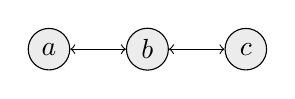
\begin{tikzpicture}
  \foreach \pos/\name in {{(0,0)/a}, {(1.25,0)/b}, {(2.5,0)/c}}
        \node (\name) at \pos {$\name$};
   \foreach \from/\to in {a/b, b/c}
	\draw [<->] (\from) -- (\to);
\end{tikzpicture}

&

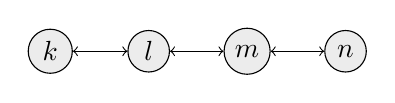
\begin{tikzpicture}
  \foreach \pos/\name in {{(0,0)/k}, {(1.25,0)/l}, {(2.5,0)/m}, {(3.75,0)/n}}
        \node (\name) at \pos {$\name$};
   \foreach \from/\to in {k/l, l/m, m/n}
	\draw [<->] (\from) -- (\to);
\end{tikzpicture}

&

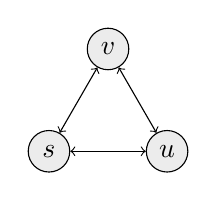
\begin{tikzpicture}
%[scale=1, transform shape]
  \foreach \pos/\name in {{(0,0)/s}, {+(0: 1.5)/u}, {+(60: 1.5)/v}}
        \node (\name) at \pos {$\name$};
   \foreach \from/\to in {s/u, u/v, v/s}
	\draw [<->] (\from) -- (\to);
\end{tikzpicture}

\end{tabular}

\vspace{-5pt}
\caption{{Simple graphs on which our example patrolling games are played.}}
\label{fig:examples}
\end{figure}

\vspace{-5pt}
\begin{example}
\label{ex:stationary}
Consider a patrolling game played on the left graph from Fig.~\ref{fig:examples}, where all nodes are targets, $a$ is the initial node and $d = 4$.
The defender has to move to the node $b$ from both nodes $a$ and $c$.
All that the defender has under control is what she does in the node $b$.
If we restrict the defender's strategies to be stationary, the best value the defender can achieve is 3/4, when she goes from $b$ to $a$ with the same probability as from $b$ to $c$, i.e. with probability 1/2.
However, the defender can protect all the targets with probability 1 with a simple deterministic strategy $\sigma^*$ resulting in a run $(abcb)^\omega$.
Note that $\sigma^*$ depends only on the last two nodes---when the defender is in the node $b$, she moves to the node she has not visited in the last two steps.
\end{example}

\begin{example}
\label{ex:initial}
Now consider a patrolling game played on the middle graph from Fig.~\ref{fig:examples}, where $T = {m, n}$ and $d = 2$ and let us suppose that any node can be the initial node, not just the targets.
The value of the game clearly depends on the initial node.
If $k$ is the initial node, the attacker attacks $n$ as soon as possible and the defender has no chance to intercept this attack, i.e. $val_k = 0$.
Otherwise, the defender can defend both targets with probability 1.

Considering a general game, an interesting question arises: for which node(s) $u \in U$ does it hold that $val_u =$ max$_{v \in U} val_v$?
We show that, in general, all target nodes satisfy this condition, i.e. no initial node would yield higher value of a game than any initial target node.
This is a corollary of Lemma \ref{lem:value} and the reason why we enforce the initial node to be a target.
\end{example}

\begin{example}
\label{ex:triangle}
Consider a patrolling game played on the right graph (triangle) from Fig.~\ref{fig:examples}, where all nodes are targets, $s$ is the initial node and $d = 2$.
This example is rather sofisticated than the previous two, because the defender cannot protect all the targets with probability 1.
A simple defender's strategy that comes to one's mind is to choose the next node uniformly, i.e. with probability 1/2.
The value of this strategy is 1/2---attacker's best response is to attack a target when the defender leaves it.
One can show that this strategy is optimal among all stationary strategies.
%TODO - ref to proof
However, consider a strategy $\sigma^*$ which chooses the previously visited node with probability $(\sqrt{5} - 1)/2$ and the other node with the remaining probability $(3-\sqrt{5})/2$.
In the first step, when there is no previously visited node, $\sigma^*$ chooses the next node uniformly.
It is easy to show that $val(\sigma^* = (\sqrt{5} - 1)/2$.
In \cite{iti1}, it has been shown that $val(\sigma^*) = val$ and that all optimal strategies are the same as $\sigma^*$ except for the choice in the first step.
%TODO - own proof?
This means that irrational numbers may inevitably occur in both the probability distribution of the defender's strategy and the value of the game.

The last thing we want to demonstrate on this example is that if the defender had the information whether the attacker has already attacked or not, she could commit to a strategy resulting in a higher value.
Indeed, assume that the defender chooses the next node uniformly until she gets the information about an initiated attack.
At that moment, she goes to the previously visited node with probability 2/3 and to the other node with probability 1/3.
Note that this way the defender intercepts any attack with probability 2/3, which is strictly greater than $(\sqrt{5} - 1)/2$.
What is interesting about this observation is not that an additional information could help the defender, rather why this particular information would help the defender.
The reason resides in the nature of patrolling games, specifically that the defender has to think in to the future more than just $d$ steps ahead.
If she had the information about an initiated attack, she would need not to care about the future and could act in a way that would otherwise afford the attacker the opportunity to successfully attack with higher probability.
\end{example}

\chapter{Existence of Optimal Strategies}

In this chapter, we summarize the essential results achieved in \cite{iti1}, while we primarily focus on the constructs on which our results are based.

We start by defining and describing a stochastic game.
Then, we translate a given patrolling game $\mathcal{G}$ into a turn-based perfect-information stochastic safety game $\mathcal{S}$, where the defender corresponds to the maximizer.
We state that the maximizer has an optimal strategy in $\mathcal{S}$, which can be translated back to $\mathcal{G}$, yielding the same value of the game.
We skip some technical parts (mostly proofs) which can be found in \cite{iti1}.

\section{Translating Patrolling Games into Stochastic Games}

\begin{definition}
%$(V_\Diamond, V_\square)$ - Diamond = Min, Square = Max
%TODO Min / Max v definiciach/lemmatoch je sam o sebe \emph, takze neviem, ci to treba znova
A \emph{stochastic game} is a tuple $\mathcal{S} = (V, (V_{\emph{Min}}, V_{\emph{Max}}), \ell, A, \mathbf{E}, \mathbf{P})$ where $V$ is a set of \emph{vertices}, $(V_{\emph{Min}}, V_{\emph{Max}})$ is a partition of $V$, $\ell \in \mathbb{N}$, $A \subseteq \mathbb{R}^\ell$ is a set of \emph{actions}\footnote{
The reason why actions are defined as real-valued vectors of a fixed dimension becomes clear later.
Such a set of actions satisfies certain conditions which are used to prove the existence of an optimal strategy for player \emph{Max}.}, $\mathbf{E} : V \to 2^A$ assigns to each vertex a set of \emph{enabled actions}, and $\mathbf{P} : V \times A \to \Delta(V)$ assigns to each $(v, a) \in V \times A$ a discrete probability distribution over $V$ with finite support.
%TODONE: each $(v, a), v \in V, a \in E(v)$ 
\end{definition}
%TODONE: $P(v, a)$ is relevant only for $a \in E(v)$
A stochastic game $\mathcal{S}$ is played between two players, \emph{Min} and \emph{Max}.
A play of $\mathcal{S}$ starts in some vertex $u \in V$ and then proceeds to other vertices based on the actions chosen.
Player $\bigcirc \in \{\emph{Min}, \emph{Max}\}$ chooses actions in the vertices of $V_\bigcirc$.
When the play is in a vertex $v \in V_\bigcirc$ and player $\bigcirc$ selects an action $a \in \mathbf{E}(v)$, the next node is chosen randomly according to the distribution $\mathbf{P}(v, a)$.
Players can choose actions based on all the vertices already visited, not just the current one.
However, the players cannot randomize.\footnote{As we will see, for our purposes of translation between patrolling and stochastic games, players in stochastic games need not to randomize---for every vertex $v \in V_{\emph{Max}}$, the set of enabled actions $\mathbf{E}(v)$ will be closed under convex combination, and the attacker cannot randomize even in patrolling games.}
Formally, a \emph{strategy} for player $\bigcirc \in \{\emph{Min}, \emph{Max}\}$ is a function $\theta_\bigcirc : V^*V_\bigcirc \to A$ satisfying $\theta_\bigcirc (wv) \in \mathbf{E}(v)$ for all $w \in V^*$ and $v \in V_\bigcirc$.

Similarly to patrolling games, every initial vertex $v \in V$ and every pair of players' strategies $(\theta_{\emph{Min}}, \theta_{\emph{Max}})$ determine a unique probability space over all infinite sequences of vertices starting in $v$ (see \cite{chung}).
Given an initial vertex $v \in V$, a target vertex $t \in V$, and a pair of players' strategies $(\theta_{\emph{Min}}, \theta_{\emph{Max}})$, we denote by $val^\mathcal{S}(\theta_{\emph{Min}}, \theta_{\emph{Max}}, v, t)$ the probability of all infinite sequences of vertices starting in $v$ that \emph{never} visit $t$.
We define $val^\mathcal{S}(\theta_{\emph{Max}}, v, t) = \inf_{\theta_{\emph{Min}}}val^\mathcal{S}(\theta_{\emph{Min}}, \theta_{\emph{Max}}, v, t)$. Furthermore, we define \linebreak
$val^\mathcal{S}(v, t) = \sup_{\theta_{\emph{Max}}}val^\mathcal{S}(\theta_{\emph{Max}}, v, t)$.
Given a target $t \in V$, a strategy $\theta_{\emph{Max}}^*$ is called \emph{optimal} if $val^\mathcal{S}(\theta_{\emph{Max}}^*, v, t) = val^\mathcal{S}(v, t)$ for all $v \in V$.

\

Now we present the idea behind the translation of imperfect-information patrolling games into perfect-information stochastic games.
Patrolling \linebreak games employ the Stackelberg model, where the defender first commits to a strategy and has no knowledge about the attacker, whereas the attacker has complete knowledge about the defender's strategy and her current position.
As we have seen in Example \ref{ex:triangle}, it is crucial that the defender cannot exploit the knowledge that the attacker has already attacked.
To cope with this restriction, we define the stochastic game in a way that the vertices correspond to defender's $d$-step randomized plans, where $d$ is the attack length.
The actions of player \emph{Max} correspond to selecting and prolonging these plans and the actions of player \emph{Min} correspond to attacker's decisions whether to attack some target or not.
When player \emph{Min} chooses an action corresponding to attacking a target, the outcome of the game is immediately computed based on the fixed $d$-step plan, and the players can make no more choices afterwards.
When player \emph{Min} chooses the action corresponding to attacker's waiting, player \emph{Max} has to prolong 
the previously fixed $d$-step plan by one step and the first step of the plan is performed, so it remains a $d$-step plan.\footnote{Although it would be sufficient to first perform the first step of the plan, and then prolong it by one step, we prefer to be consistent with \cite{iti1}.}
%jedine dolezite je, aby bol fixnuty d-commitment, ked ma hrac Min moznost zautocit

%TODONE - do we need this? if yes, do we need it here?
%In \cite{iti2}, it has been shown that if the defender uses a given strategy $\sigma$, there is an attacker's best response strategy $\pi$ which attacks with probability 1.
%Therefore, (in the rest of this chapter/section) we assume that the attacker attacks with probability 1.
%(plays according to such a strategy)

After informal description of the translation process, let us become more precise.
We start by formalizing the concept of a $k$-step randomized plan.
Let us fix a patrolling game $\mathcal{G} = (U, E, T, \hat{u}, d)$.

\begin{definition}
Let $k \in \mathbb{N}$. A \emph{$k$-commitment} is a function $f : U^{\leq k} \to \Delta(U)$ satisfying the following conditions:
\vspace{-5pt}
\begin{itemize}
	\item $f(\epsilon)(u) = 1$ for some $u \in U$,
	\item $supp(f(wu)) \subseteq succ(u)$ for all $w \in U^{\leq k - 1}$ and $u \in U$.
\end{itemize}
\vspace{-5pt}
The \emph{root} of a commitment $f$, denoted by $r(f)$, is the unique node $u$ satisfying $f(\epsilon)(u) = 1$.
We denote by $\mathbf{Comm}_k$ and $\mathbf{Comm}_k(u)$ the sets of all $k$-commitments and of all $k$-commitments $f$ with $r(f) = u$, respectively.
Further, we define $\xi(f) = f(r(f))$ to be the probability distribution in the root of $f$.
\end{definition}

A given $d$-commitment $f$ can be interpreted as a Markov chain with $U^{\leq d+1}$ as the set of states and the transition probabilities given by $f$ (the states of $U^{d+1}$ are absorbing).
Once the defender is in a node $u$ and a $d$-commitment $f \in \mathbf{Comm}_d(u)$ is fixed, the probability of detecting an immediate attack on a target can be computed in the following way.
For every $d$-commitment $f$ and every target $t \in T$, we define the value $val(f, t)$ of defending target $t$ with commitment $f$ as the probability of reaching a state of the form $wt, w\neq \epsilon$,
from state $\epsilon$ in the Markov chain induced by $f$.
Further, we define $val(f) = \text{min}_{t\in T} ~val(f, t)$.

The concept of extending a $d$-commitment is quite intuitive.
Given a $d$-commitment $f$ and a $d+$1-commitment $g$, we say that $g$ \emph{extends} $f$ if for every $w \in U^{\leq d}$ we have that $g(w) = f(w)$.
Further, we say that a $d$-commitment $f'$ is the \emph{$u$-suffix} of $g$ if $r(f') = u$ and for every $w \in U^{\leq d-1}$ we have that $f'(uw) = g(r(g)uw)$.
Player \emph{Max}'s new $d$-step plan is actually a $u$-suffix of an extension of her original plan.

Now follows the translation of the patrolling game $\mathcal{G}$ to a stochastic game, as presented in \cite{iti1}.
We define a stochastic game $\mathcal{S} = (V, (V_{\emph{Min}}, V_{\emph{Max}}),$ $|U|^{d+2}, A, \mathbf{E}, \mathbf{P})$ where players \emph{Min} and \emph{Max} correspond to the attacker and defender in $\mathcal{G}$, respectively.
\vspace{-5pt}
\begin{itemize}
	\item $V = (\{\emph{Min}, \emph{Max}\} \times \mathbf{Comm}_d) \cup \{\mathit{init}, \mathit{succ}, \mathit{fail}\}$
	\item $V_{\emph{Min}} = (\{\emph{Min}\} \times \mathbf{Comm}_d)$
	\item $V_{\emph{Max}} = (\{\emph{Max}\} \times \mathbf{Comm}_d) \cup \{\mathit{init}, \mathit{succ}, \mathit{fail}\}$
	\item $A = \mathbf{Comm}_d \cup \mathbf{Comm}_{d+1} \cup T \cup \{\perp\}$
	\item the action enabling function $\mathbf{E}$ is defined as follows:
	\vspace{-4pt}
	\begin{itemize}
		\item $\mathbf{E}(\mathit{init}) = \mathbf{Comm}_d(\hat{u}), \mathbf{E}(\mathit{succ}) = \mathbf{E}(\mathit{fail}) = \{\perp\}$ 
		\item $\mathbf{E}((\emph{Min}, f)) = T \cup \{\perp\}$ 
		\item $\mathbf{E}((\emph{Max}, f)) = \{g \in \mathbf{Comm}_{d+1} \mid g~\text{extends}~f\}$ 
	\end{itemize}
	\vspace{-4pt}
	\item the function $\mathbf{P}$ is defined as follows:
	\vspace{-4pt}
	\begin{itemize}
		\item $\mathbf{P}(\mathit{init}, f)((\emph{Min}, f)) = 1$
		\item for $(\emph{Min}, f) \in V_{\emph{Min}}$ we put
		\vspace{-2pt}
		\begin{itemize}
			\item $\mathbf{P}((\emph{Min}, f), \perp)((\emph{Max}, f)) = 1$
			\item $\mathbf{P}((\emph{Min}, f), t)(\mathit{succ}) = val(f, t)$
			\item $\mathbf{P}((\emph{Min}, f), t)(\mathit{fail}) = 1 - val(f, t)$
		\end{itemize}
		\vspace{-2pt}
		\item $\mathbf{P}((\emph{Max}, f), g)((\emph{Min}, f')) = \xi(f)(u)$ where $f'$ is the $u$-suffix~of~$g$
		\item $\mathbf{P}(\mathit{succ}, \perp)(\mathit{succ}) = \mathbf{P}(\mathit{fail}, \perp)(\mathit{fail}) = 1$
	\end{itemize}
	\vspace{-4pt}
\end{itemize}
\vspace{-5pt}

It remains to show that $A$ is a subset of $[0, 1]^{|U|^{d+2}}$.
Remember that a $d$-commitment can be interpreted as a Markov chain with a tree-like structure ($|U|$-ary tree of depth $d$.)
Putting the values of a $d+$1-commitment next to each other, the commitment can be seen as a vector of dimension $|U|^{d+2}$.
Coding the $d$-commitments as such vectors is straightforward and the remaining actions, $T \cup \{\perp\}$, can be mapped to arbitrary distinct vectors of $[0, 1]^{|U|^{d+2}}$ which do not represent commitments.

The process of translating a defender's strategy $\sigma$ in $\mathcal{G}$ to a strategy $\theta_{\emph{Max}}[\sigma]$ of player \emph{Max} in $\mathcal{S}$, and vice versa ($\theta_{\emph{Max}}$ to $\sigma[\theta_{\emph{Max}}]$), is described in detail in \cite{iti1}.
There, it has also been proven that this translation preserves the values of the strategies, which is captured by the following lemma.

\begin{lemma}
\label{lem:translation}
For every defender's strategy $\sigma$ in $\mathcal{G}$ we have that $val^\mathcal{S}(\theta_{\emph{Max}}[\sigma], \mathit{init},$ $\mathit{fail}) = val(\sigma)$.
Further, for every strategy $\theta_{\emph{Max}}$ of player \emph{Max} in $\mathcal{S}$ we have that $val^\mathcal{S}(\theta_{\emph{Max}}, \mathit{init}, \mathit{fail}) = val(\sigma[\theta_{\emph{Max}}])$.
\end{lemma}

In general, optimal strategies for player \emph{Max} in stochastic games may not exist---some extra conditions have to be satisfied.
In \cite{iti1}, it has been proven that $\mathcal{S}$ satisfies such sufficient conditions and there exists an optimal memoryless strategy for player \emph{Max} in $\mathcal{S}$.

Combining the upper two paragraphs, we get:
\begin{thm}
\label{thm:existence}
The defender has an optimal strategy in $\mathcal{G}$.
\end{thm}

For details of the translation process and the omitted proofs, see \cite{iti1}.

\chapter{Main Result}
In this chapter, we review and extend the results presented in \cite{iti1}.
There, the authors have proven the existence of a \emph{regular} $\epsilon$-optimal defender's strategy.
They provide an algorithm to compute a deterministic finite automaton encoding the strategy.
The size of the automaton is doubly exponential in $d$ (the attack length) and singly exponential in $|U|$ (the number of nodes).

We provide a modified algorithm for computing an $\epsilon$-optimal defender's strategy.
We are able to encode the strategy with a deterministic finite automaton whose size is only quadratically exponential in $d$ and singly exponential in $|U|$.

\section{Properties of Optimal Strategies in Patrolling Games}
\label{sec:value}
In this section, we examine the properties of a defender's strategy after a history has been played.
We summarize them in one powerful lemma from \cite{iti1} for which we provide a much simpler proof.

\begin{definition}
Let $\sigma$ be a defender's strategy and $h$ a history.
We define a strategy $\sigma_h$ by $\sigma_h(last(h)h') = \sigma(hh')$ for all $h' \in U^*$.
Further, we define the value of $\sigma$ after the history $h$ has been played by $val(\sigma \mid h) = val_{last(h)}(\sigma_h)$.
\end{definition}

The following lemma from \cite{iti1} states that each optimal strategy retains its value throughout a play of the game.
This knowledge is crucial in our argumentation about $\epsilon$-optimality in the next section.

\begin{lemma}
\label{lem:value}
Let $\sigma$ be an optimal defender's strategy and $h \in \mathcal{H}(\sigma)$ a history.
We have that $val(\sigma \mid h) = val(\sigma)$.
\end{lemma}
\begin{proof}
The value of the game might depend on the initial node.
Let us denote by $\mathcal{G}_u$ the patrolling game derived from $\mathcal{G}$ by changing the initial node to~$u$.
Let us consider a game $\mathcal{G}_v$ with the largest value among all such games $\mathcal{G}_u$, i.e. $val_v = \max_{u \in U} val_u$, and let $\sigma^v$ be an optimal defender's strategy in $\mathcal{G}_v$.
Clearly, for all defender's strategies $\sigma' \in \Sigma$ and all histories $h \in \mathcal{H}(\sigma')$ we have that $val(\sigma' \mid h) \leq val_v$.
Otherwise, $val_{last(h)}$ would be strictly greater than $val_v$---a contradiction.

However, as $val(\sigma^v \mid h)$ cannot be greater than $val(\sigma^v)$ for any relevant history $h$, it cannot be less than $val(\sigma^v)$ either as that would necessarily decrease the value of $\sigma^v$.
Therefore, $val(\sigma^v \mid h) = val(\sigma^v)$ for all $h \in \mathcal{H}(\sigma^v)$.
Formally, this follows from the observation that the value of $\sigma^v$ cannot decrease if we do not allow the attacker to attack in the first $k \in \mathbb{N}$ steps, which is used in the first inequality here:
$$val(\sigma^v) \leq \sum_{h \in \mathcal{H}(\sigma^v) \wedge |h| = k}(val(\sigma^v \mid h)) \cdot P^{\sigma^v}(\mathcal{R}(h))) \leq val(\sigma^v)~.$$
The second inequality follows from the fact that $val(\sigma^v\mid h) \leq val(\sigma^v)$ for all $h \in \mathcal{H}(\sigma^v)$, and the fact that $\sum_{h \in \mathcal{H}(\sigma^v) \wedge |h| = k} P^{\sigma^v}(\mathcal{R}(h)) = 1$ for all $k \in \mathbb{N}$.

Note that unless $val_v = 0$, there exists a history $h' \in \mathcal{H}(\sigma^v)$ such that $last(h') = \hat{u}$.
This history $h'$ determines a strategy $\sigma^v_{h'}$ in $\mathcal{G}$.
It follows that $val \geq val(\sigma^v_{h'}) = val_v \geq val$, i.e. $val = val_v$.
Using the same argumentation as before, we get that $val(\sigma \mid h) = val(\sigma)$ for all optimal defender's strategies $\sigma$ and all histories $h \in \mathcal{H}(\sigma)$.
\end{proof}

Note that Lemma \ref{lem:value} would not hold without the restriction that the initial node has to be a target (see Example \ref{ex:initial} for counterexample).
In the proof, the existence of the strategy $\sigma^v_{h'}$ depends on this restriction.

\section{Discretization and $\epsilon$-optimality}
As it is common in algorithmic game theory, we are interested in strategies implementable by finite-memory controllers.
In order to formalize this concept, we define a \emph{regular} strategy.
As stated in \cite{iti2}, a defender�s strategy $\sigma$ is \emph{regular} if there is a deterministic finite automaton (DFA) \cite{dfa} $\mathcal{A}$ over the alphabet $U$ (the set of nodes) such that $\sigma(h)$ depends only on the control state entered by $\mathcal{A}$ after reading $h$.

In the rest of this section, we prove the existence of a regular $\epsilon$-optimal defender's strategy.
We proceed in three steps.
We start with an optimal defender's strategy $\sigma$, whose existence is guaranteed by Theorem \ref{thm:existence}.
First, we discretize $\sigma$ to obtain an $\epsilon$-optimal strategy $\sigma_\epsilon$.
Second, using translation process from the previous chapter, we translate $\sigma_\epsilon$ from $\mathcal{G}$ to a strategy $\theta_\emph{Max}$ in the corresponding stochastic game $\mathcal{S}$.
As $\theta_\emph{Max}$ stays in finitely many vertices, we restrict the set of vertices of $\mathcal{S}$ to be finite.
We apply standard results for finite-state stochastic games to obtain an optimal memoryless strategy $\theta_\emph{Max}^{ml}$.
Third, using $\theta_\emph{Max}^{ml}$, we construct a DFA which encodes an $\epsilon$-optimal strategy.

\textbf{Step 1.} Let us fix an optimal defender's strategy $\sigma$, whose existence is guaranteed by Theorem \ref{thm:existence}.
For a desired precision $\epsilon$, we discretize $\sigma$ to obtain a strategy $\sigma_\epsilon$ with all probabilities $\sigma_\epsilon(h)(u)$ being integer multiples of an appropriate number $s$ satisfying \mbox{$s = 1/l$} for some $l \in \mathbb{N}$.
As we will see, to guarantee the $\epsilon$-optimality of $\sigma_\epsilon$, it suffices that $|\sigma(h)(u) - \sigma_\epsilon(h)(u)| \leq {\epsilon\over{|U|d}}$.
We can guarantee this property for $s = \lceil(|U|d)/\epsilon\rceil^{-1}$ using the following rounding procedure.

Let $U = \{u_1, u_2, \dots, u_{|U|}\}$ be the set of nodes of $\mathcal{G}$.
For every history $h$ and every $1 \leq i \leq |U|$, we inductively define $\sigma_\epsilon(h)(u_i) = k_i \cdot s$, where $k_i$  is the largest number satisfying
$$ k_i \cdot s \leq \sigma(h)(u_i) + \sum_{j=1}^{i-1}(\sigma(h)(u_j) - \sigma_\epsilon(h)(u_j))~.$$
This rounding procedure guarantees
that $\sigma_\epsilon(h)$ is indeed a probability distribution over $U$, i.e. $\sum_{u\in U}\sigma_\epsilon(h)(u) = 1$ (note that simple rounding would not guarantee this property).
Further, when we realize the invariant $0 \leq \sum_{j=1}^{i-1}(\sigma(h)(u_j) - \sigma_\epsilon(h)(u_j)) < s$ holds for all $1 \leq i \leq |U|$, it is easy to see that $|\sigma(h)(u_i) - \sigma_\epsilon(h)(u_i)| < s$, which is captured by the following lemma.
\begin{lemma}
\label{lem:difference}
For all $h \in \mathcal{H}$ and $u \in U$ we have $|\sigma(h)(u) - \sigma_\epsilon(h)(u)| < s$.
\end{lemma}

We base the proof of the $\epsilon$-optimality of $\sigma_\epsilon$ on the following two observations.
First, it follows from Lemma \ref{lem:value} that whenever the attacker attacks, the defender will capture him using $\sigma$ with probability at least as large as $val(\sigma)$.
And second, we argue that the probability of capturing the attacker in the same moment using $\sigma_\epsilon$ is at least as large as using $\sigma$ minus $\epsilon$.

To formulate this, let us start with a formal definition of the defender's value against an immediate attack after a given relevant history.

\begin{definition}
Let $\iota$ be a defender's strategy and $h \in \mathcal{H}(\iota)$ a history.
We define
$$att\text{-}val(\iota \mid h) = \inf_{t \in T} \mathcal{P}_{last(h)}^{\iota_h}(D_{last(h)}[t])$$
where $D_{last(h)}[t]$ is the set of all runs initiated in $last(h)$ that visit $t$ in the first $d$ steps.
\end{definition}

The following lemma states that any attack at any moment is captured using $\sigma_\epsilon$ with probability at least $val(\sigma) - \epsilon$.
\begin{lemma}
\label{lem:epsilon}
For every $h \in \mathcal{H}(\sigma_\epsilon)$ we have that $att\text{-}val(\sigma_\epsilon \mid h) \geq val(\sigma) - \epsilon$.
\end{lemma}

\begin{proof}
It follows from the definition of $\sigma_\epsilon$ that whenever $\sigma(h)(u) = 0$, then also $\sigma_\epsilon(h)(u) = 0$.
This means that any history executable using $\sigma_\epsilon$ is also executable using $\sigma$, i.e. $\mathcal{H}(\sigma_\epsilon) \subseteq \mathcal{H}(\sigma)$.
Now, knowing that $att\text{-}val(\sigma \mid h)$ is defined if $att\text{-}val(\sigma_\epsilon \mid h)$ is defined, we prove the following:
\begin{align}
att\text{-}val(\sigma_\epsilon \mid h)
  &\geq att\text{-}val(\sigma \mid h) - \epsilon\label{eq1:first} \\
  &\geq val(\sigma \mid h) - \epsilon\label{eq1:second} \\
  &= val(\sigma) - \epsilon\label{eq1:third}~.
\end{align}
\begin{itemize}
	\item The equality \eqref{eq1:third} directly follows from Lemma \ref{lem:value} as $\sigma$ is an optimal strategy and $h \in \mathcal{H}(\sigma)$.
	\item The inequality \eqref{eq1:second} clearly holds as restricting the attacker to attack immediately cannot decrease the value of the game.
Formally, it follows from the fact that $D_{last(h)}[t] = D_{last(h)}[\pi]$ for $\pi(last(h)) = t$.
	\item To prove the first inequality \eqref{eq1:first}, we have to analyze the impact of the rounding in the definition of $\sigma_\epsilon$.
Denote by $R[\iota, h, t, k]$ the probability of reaching $t \in T$ from $last(h), h \in \mathcal{H}$ in up to $k$ steps using the strategy $\iota_h$.
We prove by induction on $k$ that for all $h \in \mathcal{H}$, $t \in T$, and $k \in \mathbb{N}$ we have that
\begin{align}
R[\sigma, h, t, k] - R[\sigma_\epsilon, h, t, k] \leq k|U|s~.\nonumber
\end{align}

The base case ($k = 1$) directly follows from Lemma \ref{lem:difference} and the fact that $R[\iota, h, u, 1] = \iota(h)(u)$.
%The base case ($k = 0$) clearly holds as the value of $R[\iota, h, u, 0]$ is independent of the strategy $\iota$---it is $1$ if $last(h) = u$, and it is $0$ otherwise.

Let us denote the difference $R[\sigma, h, t, k] - R[\sigma_\epsilon, h, t, k]$ by $\Delta$.
For $k \geq 2$, we have
\begin{eqnarray}
\Delta
  &=& \sigma(h)(t) + \sum_{u\in U \smallsetminus \{t\}}\sigma(h)(u)\cdot R[\sigma, hu, t, k - 1] - \label{eq1b:first} \\
  & &\hspace{-11.2pt} -~\sigma_\epsilon(h)(t) - \sum_{u\in U \smallsetminus \{t\}}\sigma_\epsilon(h)(u)\cdot R[\sigma_\epsilon, hu, t, k - 1]	\nonumber \\
  &\leq& s + \sum_{u\in U \smallsetminus \{t\}}(R[\sigma, hu, t, k - 1]\cdot (\sigma(h)(u) - \sigma_\epsilon(h)(u)) \label{eq1b:second} +	\\
  & &\hspace{47.5pt} +~\sigma_\epsilon(h)(u)\cdot (R[\sigma, hu, t, k - 1] - R[\sigma_\epsilon, hu, t, k - 1])) \nonumber	 \\
  &\leq& s + \sum_{u\in U \smallsetminus \{t\}} R[\sigma, hu, t, k - 1]\cdot s + \label{eq1b:third}	\\	%\sigma_\epsilon(h)(u)\cdot (k - 1)|U|s)\label{eq1b:third}	\\
& &\hspace{7.6pt} +\hspace{-2pt}~\sum_{u\in U \smallsetminus \{t\}} \sigma_\epsilon(h)(u)\cdot (k - 1)|U|s \nonumber	\\
	%  &\hspace{5pt}+\hspace{-5pt}& \sum_{u\in U} \sigma_\epsilon(h)(u)\cdot (k - 1)|U|s \nonumber	\\
  &\leq& s + (|U|-1)s + (k - 1)|U|s	\label{eq1b:fourth} \\
  &=& k|U|s\nonumber~.
\end{eqnarray}
\begin{itemize}
	\item The equality \eqref{eq1b:first} follows from the definition of $R[\iota, h, t, k]$ as $R[\iota, h, t, k] = \iota(h)(t) + \sum_{u \in U \smallsetminus \{t\}} \iota(h)(u) \cdot R[\iota, hu, t, k - 1]$ for all $k \geq 2$. %$k \in \mathbb{N}$.
	\item The equality \eqref{eq1b:second} is just an application of Lemma \ref{lem:difference} and of the formula $ab - a'b' = b(a -  a') + a'(b - b')$.
	\item The inequality \eqref{eq1b:third} follows from Lemma \ref{lem:difference} and from the induction hypothesis.
	\item The inequality \eqref{eq1b:fourth} holds because $R[\sigma, hu, t, k - 1] \leq 1$ and $\sum_{u\in U \smallsetminus \{t\}} \sigma_\epsilon(h)(u) \leq 1$.
\end{itemize}
So we have that $R[\sigma, h, t, d] - R[\sigma_\epsilon, h, t, d] \leq d|U|s$.
However, note that
$$att\text{-}val(\iota \mid h) = \inf_{t \in T} R[\iota, h, t, d]$$
and therefore
$$att\text{-}val(\sigma \mid h) - att\text{-}val(\sigma_\epsilon \mid h) \leq d|U|s \leq \epsilon~.$$
\end{itemize}
\end{proof}

A trivial implication of Lemma \ref{lem:epsilon} is that 
$\sigma_\epsilon$ is an $\epsilon$-optimal strategy,
as $val(\sigma_\epsilon) \geq \inf_{h \in \mathcal{H}(\sigma_\epsilon)} att\text{-}val(\sigma_\epsilon \mid h) \geq val(\sigma) - \epsilon$.

\textbf{Step 2.}
According to Lemma \ref{lem:translation}, we can translate the strategy $\sigma_\epsilon$ in $\mathcal{G}$ to a strategy $\theta_{\emph{Max}} := \theta_{\emph{Max}}[\sigma_\epsilon]$ in $\mathcal{S}$ such that
$$val^\mathcal{S}(\theta_\emph{Max}, \mathit{init}, \mathit{fail}) = val(\sigma_\epsilon)~.$$
Let us denote by $\mathbf{Reach}(\theta_\emph{Max})$ the set of all vertices in $\mathcal{S}$ that are reachable from $\mathit{init}$ using $\theta_\emph{Max}$.
Note that for every $(\bigcirc, f) \in \mathbf{Reach}(\theta_\emph{Max})$, $w \in U^{\leq d}$ and $u \in U$ we have that $f(w)(u)$ is an integer multiple of $t$.
As there are only finitely many such commitments $f$, the set $\mathbf{Reach}(\theta_\emph{Max})$ is finite.

By restricting the set of vertices of $\mathcal{S}$ to $\mathbf{Reach}(\theta_\emph{Max})$, we obtain a stochastic game $\mathcal{S}_\epsilon$.
As $\theta_{\emph{Max}}$ is a valid strategy in $\mathcal{S}_\epsilon$, we have
$$val^{\mathcal{S}_\epsilon}(\theta_\emph{Max}, \mathit{init}, \mathit{fail}) = val^\mathcal{S}(\theta_\emph{Max}, \mathit{init}, \mathit{fail})~.$$
Applying results for perfect-information stochastic games with finitely many states (see \cite{kucera}), we obtain an optimal memoryless\footnote{A \emph{memoryless} strategy depends only on the current vertice. Therefore, a memoryless strategy for player \emph{Max} can be defined as a function $\theta_\emph{Max}^{ml} : V_\emph{Max} \to A$.} strategy $\theta_\emph{Max}^{ml}$ such that
$$val^{\mathcal{S}_\epsilon}(\theta_\emph{Max}^{ml}, \mathit{init}, \mathit{fail}) \geq val^{\mathcal{S}_\epsilon}(\theta_\emph{Max}, \mathit{init}, \mathit{fail})~.$$
As $\mathbf{Reach}(\theta_\emph{Max})$ is a subset of vertices of $\mathcal{S}$, $\theta_\emph{Max}^{ml}$ is a valid strategy in $\mathcal{S}$ and we have
$$val^\mathcal{S}(\theta_\emph{Max}^{ml}, \mathit{init}, \mathit{fail}) = val^{\mathcal{S}_\epsilon}(\theta_\emph{Max}^{ml}, \mathit{init}, \mathit{fail})~.$$
Summing up, $\theta_\emph{Max}^{ml}$ is a memoryless strategy
satisfying
$$val^\mathcal{S}(\theta_\emph{Max}^{ml}, \mathit{init}, \mathit{fail}) \geq val(\sigma_\epsilon)~.$$

\textbf{Step 3.}
Using $\theta_\emph{Max}^{ml}$, we construct a DFA $\mathcal{A}$ encoding the desired regular \hbox{$\epsilon$-optimal} strategy $\sigma_\epsilon^{reg}$ as follows: $\mathcal{A} = (Q, U, \delta, q_0, \emptyset)$ where
\vspace{-3pt}
\begin{itemize}
	\item $Q = \{f \mid (\emph{Max}, f) \in \mathbf{Reach}(\theta_\emph{Max})\}$ is the finite set of states
	\item $U$ is the alphabet, %a finite set of input symbols,
	\item $\delta : Q \times U \to Q$ is a transition function such that
$\delta(f, u) = f'$ where $f'$ is the $u$-suffix of $\theta_\emph{Max}^{ml}((\emph{Max}, f))$,\footnote{Note that $\theta_\emph{Max}^{ml}$ takes as an argument only a single vertex. That would not be possible unless $\theta_\emph{Max}^{ml}$ was a memoryless strategy.}
	\item $q_0 = \theta_\emph{Max}^{ml}(init)$ is the initial state.
\end{itemize}
\vspace{-3pt}
For a history $h$, we denote by $h^+$ the word equal to $h$ without its first letter, i.e. $h = h_0h^+$.
We denote by $\mathcal{A}[h^+]$ the state of $\mathcal{A}$ reached after reading the word $h^+$.
We define $\sigma_\epsilon^{reg}(h) = \xi(\mathcal{A}[h^+])$ (recall that $\xi(f) = f(r(f))$ for a commitment $f$).
It is easy to show that $\sigma_\epsilon^{reg}$ is the same as $\sigma[\theta_\emph{Max}^{ml}]$ obtained from $\theta_\emph{Max}^{ml}$ using Lemma \ref{lem:translation}.
It follows that
$$val(\sigma_\epsilon^{reg}) = val^\mathcal{S}(\theta_\emph{Max}^{ml}, \mathit{init}, \mathit{fail}) \geq val(\sigma_\epsilon) \geq val(\sigma) - \epsilon~,$$
i.e. $\sigma_\epsilon^{reg}$ is $\epsilon$-optimal.

%IDEA oddelit riadkom navyse?

Before we move to the next section, we show one important observation about the states of the automaton $\mathcal{A}$.
Based on the properties of the translation process from $\mathcal{G}$ to $\mathcal{S}$, we know that $\theta_{\emph{Max}}$ encodes exactly the same defender's strategy as $\sigma_\epsilon$.
When we realize that $Q$ is the set of all $d$-commitments $f$ occuring in vertices of $\mathbf{Reach}(\theta_\emph{Max})$, it is easy to get the following statement using Lemma \ref{lem:epsilon}.

\begin{lemma}
\label{lem:epsilon_commitment}
For every $d$-commitment $f \in Q$, we have that $val(f) \geq val(\sigma) - \epsilon$.
\end{lemma}

\section{Characteristics}

As you may noticed, the above proof of existence of an $\epsilon$-optimal strategy is not constructive.
In \cite{iti1}, the authors provide an algorithm which computes the desired strategy.
They introduce the concept of a \emph{discretized} $d$-commitment $f$ for which it holds that for all $w \in U^{\leq d}$ and $u \in U$ the number $f(w)(u)$ is an integer multiple of $t$.
Their algorithm is based on searching for a \emph{closed} set of such commitments (the defender stays within this set by prolonging her plans) that maximizes the minimal value of all commitments.
It runs in time polynomial in the number of all discretized $d$-commitments, i.e. in time ${\left({{d\cdot|U|}\over \epsilon}\right)}^{|U|^{\mathcal{O}(d)}}$.
We provide a stronger result:

\begin{thm}
\label{thm:complexity}
Let $\epsilon > 0$.
There is a regular $\epsilon$-optimal defender's strategy computable in time
$\left(\frac{d\cdot|U|}{\epsilon}\right)^{\mathcal{O}(d^2\cdot|U|^2)}$.
\end{thm}

To reduce the number of possible states of the automaton $\mathcal{A}$ encoding the $\epsilon$-optimal strategy, we define an equivalence relation on the states of $\mathcal{A}$ which we use to factorize the state-space of $\mathcal{A}$.
The equivalence relation is based on the ability to defend an attack which started somewhen in the last $d$ steps.
We call this ability the \emph{characteristic} of a given state.
We prove that states with the same characteristic are equivalent, i.e. they can be merged into a single state without influencing the value of the resulting strategy.

Before we define the characteristic of a given state, we start by defining a characteristic as a general function.

\begin{definition}
A \emph{characteristic} is a function $c : \{0, \dots, d\} \times U \to [0, 1]$ such that there is a unique node $u \in U$ for which the following conditions are satisfied:
\vspace{-5pt}
\begin{itemize}
	\item $c(0, u) = 1$,
	\item $c(0, v) = 0$ for all $v \in U \smallsetminus \{u\}$,
	\item $c(1, v) = 0$ for all $v \notin succ(u)$,
	\item $\sum_{v\in U}c(1, v) = 1$.
\end{itemize}
\vspace{-5pt}
This unique node $u$ is called the \emph{root} of the characteristic $c$.
%We denote by ... the set of all characteristics.
%We denote by $\psi_c \in \Delta(U)$ the probability distribution over the nodes defined as $\psi_c(u) = c(1, u)$.
\end{definition}
\noindent
%In the following definition, we assume the automaton $\mathcal{A}$ constructed in Step~3 in the previous section.
\begin{definition}
%TODO
Let $\mathcal{A} = (Q, U, \delta, q_0, \emptyset)$ be an automaton encoding a defender's strategy.
Given $p \in Q$, we define the characteristic $\mathbf{Char}_p$ of the state $p$ to be a characteristic which to every pair $(k, u) \in \{0, \dots, d\} \times U$ assigns the probability of reaching $u$ in at most $k$ steps whenever the strategy is in the state $p$ (recall that $p$ determines the current state of the play).
\end{definition}
\noindent
The root of the characteristic represents the current location of the defender
and the values for $k = 1$ represent the probability distribution over the nodes in the next step.
%For a characteristic $c$, we denote this probability distribution as $\psi_c$ and we put $\psi_c(u) = c(1, u)$.
%Given $p \in Q$, we define the characteristic $\mathbf{Char}_p$ of the state $p$ to be a characteristic defined as follows:

Note that for the automaton $\mathcal{A}$ constructed in Step~3 in the previous section, we have
\vspace{-5pt}
\begin{itemize}
	\item
\hspace{17.2pt}$\mathbf{Char}_p(0, u) =
   \begin{cases}
   1		& \text{if } r(p) = u \\
   0		& \text{otherwise}
   \end{cases}$
	\item and for $1 \leq k \leq d$
$$\mathbf{Char}_p(k, u) = \xi(p)(u) + \sum_{v \in U \smallsetminus \{u\}}\xi(p)(v) \cdot \mathbf{Char}_{\delta(p, v)}(k - 1, u)~.$$
\end{itemize}
\vspace{-5pt}
%%%%%%%%%%%%%%
%%% COMMENTED OUT %%%
% correct as the fact that it is a characteristic implies that $k \leq d$
%\noindent
%$\mathbf{Char}_p(k, u) =
%   \begin{cases}
%      \begin{cases}
%         1	& \text{if } r(p) = u \\
%         0	& \text{if } r(p) \neq u \\
%      \end{cases}
%		& \text{if } k = 0 \\
%   \xi(p)(u) + \sum_{v \in U \smallsetminus \{u\}}\xi(p)(v) \cdot \mathbf{Char}_{\delta(p, v)}(k - 1, u)	& \text{otherwise.}
%   \end{cases}$
%
%\noindent
%$\mathbf{Char}_p(k, u) =
%   \begin{cases}
%   \text{the boolean value of } r(p) = u		& \text{if } k = 0 \\
%   \xi(p)(u) + \sum_{v \in U \smallsetminus \{u\}}\xi(p)(v) \cdot \mathbf{Char}_{\delta(p, v)}(k - 1, u)	& \text{otherwise.}
%   \end{cases}$
%\end{definition}
%\noindent
%$\mathbf{Char}_p$ assigns to every pair $(k, u) \in \{0, \dots, d\} \times U$ the probability of reaching $u$ in at most $k$ steps whenever the strategy is in the state $p$ (recall that $p$ determines the current state of the play).
Observe that $\mathbf{Char}_p(1, u) = \xi(p)(u)$ because for all $v \in U \smallsetminus \{u\}$ it holds that $\mathbf{Char}_{\delta(p, v)}(0, u) = 0$.

%The current location of the defender is determined by the only node $u$ for which $\mathbf{Char}_p(0, u) = 1$ and the probability distribution over the nodes in the next step is represented by values of $\mathbf{Char}_p(1, u)$.

\

Now we describe the concept of merging two states of an automaton.
Given $q \in Q \smallsetminus \{q_0\}$, we denote by $\mathcal{A}_{p \leftarrow q} = (Q', U, \delta', q_0, \emptyset)$ the DFA defined as follows:
\vspace{-5pt}
\begin{itemize}
	\item $Q' = Q \smallsetminus \{q\}$
	\item $\delta'(r, u) =
  \begin{cases}
   p		& \text{if } \delta(r, u) = q \\
   \delta(r, u)	& \text{otherwise.}
  \end{cases}$
\end{itemize}
\vspace{-5pt}

Intuitively, $\mathcal{A}_{p \leftarrow q}$ is obtained from $\mathcal{A}$ by redirecting all transitions going to $q$ to $p$ and then removing $q$.

In general, this change in the transition function might influence the characteristics of the states from which $q$ was reachable in less than $d$ steps.
However, the states' characteristics are preserved if the two merged states have the same characteristic, as is formulated in the following lemma.

\begin{lemma}
\label{lem:characteristics}
Given $p, q \in Q$ such that $\mathbf{Char}_p = \mathbf{Char}_q$, we have that for all $r \in Q \smallsetminus \{q\}$
$$\mathbf{Char}'_r = \mathbf{Char}_r$$
where $\mathbf{Char}'_r$ denotes the characteristic of $r$ in the automaton $\mathcal{A}_{p \leftarrow q}$.
\end{lemma}

\begin{proof}
Observe that the automaton $\mathcal{A}$ together with the strategy it determines can be seen as a Markov Chain.
Indeed, when the play is in a state $f$, the next state $g$ is chosen with probability $\sum_{u \in U, g = \delta(f, u)} \xi(f)(u)$.
%TODO remove the reasoning
This is because the next node $u$ visited by the defender is selected based on $\xi(f)$, and $g$ is determined by $\delta(f, u)$.

That means that although the states of $\mathcal{A}$ are $d$-commitments, only the probability distribution in their root affects the strategy.
The idea of the proof is that the characteristic of a state $r$ is completely determined by
(1) the probability distribution in its root and by
%, by the transitions from it,
(2) the characteristics of all the states to which there is a transition from $r$ under a particular node~$u$.
%TODO dat to ako odrazky?
%\vspace{-6.1pt}
%\begin{enumerate}
%	\item the probability distribution in its root, and
%	\item the characteristics of all the states to which there is a transition from $r$ under a particular node $u$.
%\end{enumerate}
%\vspace{-6.1pt}
Substitution of $q$ by $p$ does not have any influence on (1) and because $\mathbf{Char}_p = \mathbf{Char}_q$, neither has it any influence on (2).
%Note that the characteristic of a state preserves the information about the probability distribution in its root.

%IDEA change the order of $r, v, k$
Formally, we prove by induction on $k$ that for all $r \in Q \smallsetminus \{q\}$, $v \in U$, $0 \leq k \leq d$ we have that $$\mathbf{Char}'_r(k, v) = \mathbf{Char}_r(k, v)~.$$
For $k = 0$ this clearly holds as the root of any state remains unchanged.

Now all we need is to realize that $\xi(r)$ is the same in both $\mathcal{A}$ and $\mathcal{A}_{p \leftarrow q}$.
For $1 \leq k \leq d$ we have
\begin{align}
\mathbf{Char}'_r(k, v)
  &= \xi(r)(v) + \sum_{u \in U \smallsetminus \{v\}}\xi(r)(u) \cdot \mathbf{Char}'_{\delta'(r, u)}(k - 1, v)\label{eq2:first} \\
  &= \xi(r)(v) + \sum_{u \in U \smallsetminus \{v\}}\xi(r)(u) \cdot \mathbf{Char}_{\delta'(r, u)}(k - 1, v)\label{eq2:second} \\
  &= \xi(r)(v) + \sum_{u \in U \smallsetminus \{v\}}\xi(r)(u) \cdot \mathbf{Char}_{\delta(r, u)}(k - 1, v)\label{eq2:third} \\
  &= \mathbf{Char}_r(k, v)\label{eq2:fourth}~.
\end{align}
\vspace{-20pt}
\begin{itemize}
	\item The equalities \eqref{eq2:first} and \eqref{eq2:fourth} follow directly from the definition of the characteristic of a state. %and the fact that $\mathbf{Char}_{\delta(r, u)}(0, v) = 0$ for all $u \neq v$.
	\item The equality \eqref{eq2:second} holds by the induction hypothesis.
	\item To prove the equality \eqref{eq2:third}, note that the only case when $\delta'(r, u) \neq \delta(r, u)$ is when $\delta'(r, u) = p$ and $\delta(r, u) = q$. However, $\mathbf{Char}_p = \mathbf{Char}_q$.
\end{itemize}
\vspace{-5pt}
\end{proof}
\noindent
Lemma \ref{lem:characteristics} shows that removal of one of the "equivalent" states does not influence the characteristics of the other states.
Of great importance is that the lemma holds also for the reduced automaton $\mathcal{A}_{p \leftarrow q}$.
Indeed, the proof is based only on general properties of the characteristics and on the definition of $\mathcal{A}_{p \leftarrow q}$.
%This justifies us to
This means we can repeat the process of removing equivalent states until all the states have mutually different, yet still unchanged characteristics.

Let us fix and denote by $\mathcal{A}_{red}$ %= (Q_{red}, U, \delta_{red}, q_0, \emptyset)$
the resulting automaton which cannot be further reduced by applying Lemma \ref{lem:characteristics}.\footnote{Note that the process of merging equivalent states is non-deterministic, so the resulting reduced automaton is not uniquely determined.}
We denote by $Q_{red}$ the set of states of $\mathcal{A}_{red}$ and by $\sigma_{red}$ the defender's strategy determined by $\mathcal{A}_{red}$.
In what follows, we prove that $\sigma_{red}$ is $\epsilon$-optimal.

We start by defining the probability of detecting an immediate attack when the play is in a state $p$.
\begin{definition}
Given a state $p \in Q$, we define the value of its characteristic by $$val(\mathbf{Char}_p) = \min_{t \in T} \mathbf{Char}_p(d, t)~.$$
\end{definition}
Note that $att\text{-}val(\sigma_{red} \mid h) = val(\mathbf{Char}_p)$ where $p = \mathcal{A}[h^+]$.

%%% COMMENTED OUT %%%
%Consider the automaton $\mathcal{A}$ and some $d$-commitment $p \in Q$.
%Based on the definition of $\mathcal{A}$ and $\sigma_\epsilon^{reg}$, the next $d$ steps of the play are completely determined by $p$.
%TODO vypustit historiu $h$, ak ju nepotrebujem
%Note that for a $d$-commitment $p = \mathcal{A}[h^+]$ for some history $h$, we have that $val(\mathbf{Char}_p) = val(p)$. %att\text{-}val(\sigma_\epsilon^{reg} \mid h)$.
%In other words, if the attacker attacks when the play is in a state $p$, he is caught with probability $val(\mathbf{Char}_p)$.

\newpage%TODO needed?
\begin{lemma}
\label{lem:char_value}
For each state $p \in Q$ we have $val(\mathbf{Char}_p) \geq val(\sigma) - \epsilon$.
\end{lemma}
\begin{proof}
Recall that the states are $d$-commitments and each state of the automaton $\mathcal{A}$ completely determines the next $d$ steps of the defender's strategy.\footnote{This is not true for the automaton $\mathcal{A}_{red}$ where each state determines only the next step of the defender's strategy, and the latter steps cannot be determined without the transition function.}
Therefore, we have that $val(\mathbf{Char}_p) = val(p)$.
However, $val(p) \geq val(\sigma) - \epsilon$ according to Lemma \ref{lem:epsilon_commitment}.
\end{proof}
\noindent
As $Q_{red} \subseteq Q$ and the characteristics of all the states in $\mathcal{A}_{red}$ are the same as in $\mathcal{A}$ (see Lemma \ref{lem:characteristics}), Lemma \ref{lem:char_value} provides a lower bound on the value of the characteristics of all the states of the automaton $\mathcal{A}_{red}$.
It follows that
\begin{align*}
val(\sigma_{red})
  &\geq \inf_{h \in \mathcal{H}(\sigma_{red})} att\text{-}val(\sigma_{red} \mid h) \\
  &= \inf_{h \in \mathcal{H}(\sigma_{red})} val(\mathbf{Char}_{\mathcal{A}[h^+]}) \\
  &\geq \inf_{p \in Q_{red}} val(\mathbf{Char}_p) \\
  &= \inf_{p \in Q_{red}} val(p) \\
  &\geq val(\sigma) - \epsilon
\end{align*}
i.e.
%\begin{proposition}
$\sigma_{red}$ is an $\epsilon$-optimal strategy.
%\end{proposition}

We can further substitute each state $p \in Q_{red}$ by its characteristic $\mathbf{Char}_p$ to obtain an automaton $\mathcal{A}_\mathit{Char}$.
%One can easily prove that $\mathcal{A}_\mathit{Char}$ and $\mathcal{A}_{red}$ encode exactly the same defender's %strategy.
%It suffices to put
By putting
\vspace{-5pt}
\begin{itemize}[label=-]
	\item $Q_\mathit{Char} = \{\mathbf{Char}_p \mid p \in Q_{red}\}$,
	\item $\delta_\mathit{Char}(\mathbf{Char}_p)(u) = \mathbf{Char}_q$ iff $\delta_{red}(p)(u) = q$,
	\item $\sigma_\mathit{Char}(h)(u) = \mathcal{A}_\mathit{Char}[h^+](1, u)$, %$ = \xi(\mathcal{A}_{red}[h^+])(u)$
\end{itemize}
\vspace{-5pt}
one can easily see that $\sigma_\mathit{Char} = \sigma_{red}$.

%TODO delete? dal som to k zdovodneniu pre "representable" charakteristik
%\noindent
%\textit{Remark 1. }
%When a play is in a state $p \in Q_\mathit{Char}$, there is exactly one unique $d$-commitment $f$ (determined by $\sigma_\mathit{Char}$) which represents the current $d$-step randomized plan for the defender.
%Note that it might be the case that $f \notin Q$.

%\noindent
%\textit{Remark 2. }
%We do not know whether, in general, the state-space can be bounded by the number of different probability distributions in a root, but we strongly believe it cannot.
%TODO %IDEA Napisat o $\mathcal{A}_{Char}$?

\section{The Algorithm}

So far, we have shown that there is a DFA $\mathcal{A}_\mathit{Char}$ encoding an $\epsilon$-optimal strategy such that its states $Q_\mathit{Char}$ are mutually different characteristics.
Furthermore, each $c \in Q_\mathit{Char}$ satisfies:
\vspace{-5pt}
\begin{enumerate}[label=(\Alph*)]
	\item $c = \mathbf{Char}_c$\footnote{We identify a state with its characteristic to reflect that it is the only quality of a state we are interested in.} \label{a}
	\item $c(1, u)$ is an integer multiple of $s$ for all $u \in U$, where $s = \lceil(|U|d)/\epsilon\rceil^{-1}$\label{b}
	\item $val(c) \geq val(\sigma) - \epsilon$. \label{c}
%%% COMMENTED OUT the bullets for the existence of $\mathcal{A}_{red}$ %%%
%	\item its states are $d$-commitments with all their function values (elements of probability distribution) being integer multiples of $t$,
%	\item no two states have the same characteristic, and
%	\item the value of the characteristic of each state is at least $val(\sigma) - \epsilon$.
\end{enumerate}
\vspace{-5pt}
In order to find such an automaton, we consider the set of all \emph{discretized} characteristics
$\mathit{Char}^s$ that consists of all characteristics $c$ such that $c(k, u)$ is an integer multiple of $s^k$ for all $0 \leq k \leq d$ and $u \in U$.
From \ref{a} and \ref{b} it follows that $Q_\mathit{Char} \subseteq \mathit{Char}^s$.

\begin{algorithm}[t]
\caption{~Compute an $\epsilon$-optimal strategy $\sigma_\epsilon^{alg}$}
\label{alg:algorithm1}
\begin{algorithmic}[1]
\par\vspace{0.5mm}
	\Require	Patrolling game $\mathcal{G} = (U, E, T, \hat{u}, d)$, $\epsilon > 0$
	\Ensure	a regular $\epsilon$-optimal strategy $\sigma_\epsilon^{alg}$
\par\vspace{3.5mm}

\State $C \leftarrow$ empty priority queue; $D \leftarrow \emptyset$
\State \textbf{for each} $c \in \mathit{Char}^s$ \textbf{do}
%\ForEach {$c \in \mathbf{Char}^s$}
	%\If {$c$ is \emph{representable}}	%TODO {\sum_{u \in U} $c(1, u) = 1$}, taktiez musi byt len jeden root
		add $c$ to $C$ with priority $val(c)$
%\EndFor
\vspace{3px}
\Repeat
	\State pull from $C$ the item $c$ with the highest priority
	\State $D \leftarrow D \cup \{c\}$
\Until {$D$ is \emph{complete}}	%{$complete(D)$}
\vspace{3px}
\State $\sigma_\epsilon^{alg} \leftarrow$ the strategy induced by a closed subset of $D$
\end{algorithmic}
\end{algorithm}

The algorithm we provide to compute the desired $\epsilon$-optimal strategy is a modification of the algorithm from \cite{iti1}, but instead of searching the set of discretized $d$-commitments, we search the set of discretized characteristics.
Each discretized characteristic represents a possible state of the automaton.
From these characteristics, we aim to build a DFA encoding an $\epsilon$-optimal strategy.

%When a play is in any state, there is exactly one unique $d$-commitment which represents the current $d$-step randomized plan for the defender.
%Therefore, we consider only characteristics that are \emph{representable} by some $d$-commitment---otherwise, they could not be the characteristic of any state.
%The problem of how to determine whether characteristic is representable will be addressed later.

Let $U = \{u_1, \dots, u_n\}$, $n = |U|$, be the set of nodes of $\mathcal{G}$
and let $c, c_1, \dots, c_n$ be some characteristics (not necessarily different).
We say that a sequence $(c_1, \dots, c_n)$ are \emph{successors} of $c$ if 
for all $1 \leq k \leq d$ and $u \in U$ it holds
$c(k, u) = c(1, u) + \sum_{i = 1, u_i \neq u}^n c(1, u_i) \cdot c_i(k - 1, u)$.
The meaning of this is that if, for all $i$, $c_i = \mathbf{Char}_{c_i}$ and there is a transition from the state $c$ to $c_i$ under $u_i$, then also $c = \mathbf{Char}_{c}$.
We refer to $c_i$ as the $u_i$-successor of $c$.
Note that $\sum_{i = 1, u_i \neq u}^n c(1, u_i) \cdot c_i(0, u) = 0$.
Therefore if $c(1, u_i) > 0$, then $c_i(0, u) = 0$ for all $u \neq u_i$, which implies $c_i(0, u_i) = 1$.
This guarantees that if there is a positive probability of choosing $u_i$ in the state $c$, then the root of $c_i$ is $u_i$.

We say that a non-empty set $R \subseteq \mathit{Char}^s$ is \emph{closed} if for all $c \in R$ there are successors $(c_1, \dots, c_n) \in R^n$ of $c$.
Finally, we say that a set $D \subseteq \mathit{Char}^s$ is \emph{complete} if it contains a closed subset.

Note that each closed set $R$ represents a set of states of an automaton whose transition function can be built from the states' successors.\footnote{In general, there might be several different sequences of successors for a characteristic in a closed set. Therefore, the process of building an automaton from a closed set is not deterministic.}
And for the automaton's intial state it suffices to choose some $\hat{c} \in R$ such that $\hat{c}(0, \hat{u}) = 1$.\footnote{There has to be at least one such $\hat{c} \in R$ unless the value of all characteristics from $R$ is 0.}

Let us fix a closed set $R$ and for each $c \in R$, let us fix some successors $(c_1, \dots, c_n) \in R^n$ of $c$.
Further, let us fix some $\hat{c} \in R$ such that $\hat{c}(0, \hat{u}) = 1$.
We construct a DFA $\mathcal{A}_{R} = (R, U, \delta_{R}, \hat{c}, \emptyset)$ where $\delta_{R}(c, u_i) = c_i$ for all $c \in R$ and $u_i \in U$.
%\vspace{-3pt}
%\begin{itemize}
%	\item $Q_{R} = R$ %is the finite set of states
%	%\item $U$ is the alphabet
%	\item $\delta_{R}(c, u_i) = c_i$ where $c_i$ is the fixed $u_i$-successor of $c$
%	\item $q_0 = \hat{c}$.
%\end{itemize}
%\vspace{-3pt}
We define the strategy determined by $\mathcal{A}_{R}$ as $\sigma_{R}(h)(u) = \mathcal{A}[h^+](1, u)$.
%$\sigma_{R}(h) = \psi_{\mathcal{A}[h^+]}$ (recall that $\psi_c(u) = c(1, u)$ for a characteristic $c$).
We show that for such a strategy, each state of $\mathcal{A}_{R}$ is identical with its own characteristic.

\begin{lemma}
\label{lem:char=char}
For all states $c \in R$ we have that $c = \mathbf{Char}_c$.
\end{lemma}

\begin{proof}
We prove by induction on $k$ that for all $c \in R$ and $u \in U$ it holds that $c(k, u) = \mathbf{Char}_c(k, u)$.
For $k = 0$ this trivially holds.

For $1 \leq k \leq d$, let $(c_1, \dots, c_n)$ be the successors of $c$. It follows that
\begin{align}
c(k, u)
  &= c(1, u) + \sum_{i = 1, u_i \neq u}^n c(1, u_i) \cdot c_i(k - 1, u)\label{eq3:first} \\ %from the definition of successors
  &= c(1, u) + \sum_{i = 1, u_i \neq u}^n c(1, u_i) \cdot \mathbf{Char}_{c_i}(k - 1, u)\label{eq3:second} \\ %from induction hypothesis
  &= c(1, u) + \sum_{i = 1, u_i \neq u}^n c(1, u_i) \cdot \mathbf{Char}_{\delta_{R}(c, u_i)}(k - 1, u)\nonumber \\ %%%f
  &= c(1, u) + \sum_{v \in U \smallsetminus \{u\}} c(1, v) \cdot \mathbf{Char}_{\delta_{R}(c, v)}(k - 1, u)\nonumber \\ % from the definition of characteristic of a state
  &= \mathbf{Char}_c(k, u)\label{eq3:last}~.
\end{align}
The equalities \eqref{eq3:first}, \eqref{eq3:second}, and \eqref{eq3:last} follow from the definition of successors, from the induction hypothesis, and from the definition of the characteristic of a state, respectively.
The other equalities are trivial.
%\vspace{-5pt}
%\begin{itemize}
%	\item The equality \eqref{eq3:first} follows from the definition of successors.
%	\item The equality \eqref{eq3:second} follows from the induction hypothesis.
%	\item The equality \eqref{eq3:last} follows from the definition of the characteristic of a state.
%\end{itemize}
%\vspace{-5pt}
\end{proof}

Recall that the value of the strategy determined by an automaton is bounded below by the lowest value from among the values of characteristics of the states of the automaton.
By applying Lemma \ref{lem:char=char}, it follows that $val(\sigma_{R}) \geq \min_{c \in R} val(c)$.

From the existence of the automaton $\mathcal{A}_\mathit{Char}$ %and its properties \ref{a}, \ref{b}, and \ref{c},%properties of its states
we know that there is a closed set $Q_\mathit{Char}$ such that $\min_{c \in Q_\mathit{Char}} val(c) \geq val(\sigma) - \epsilon$.
That means that in order to find an $\epsilon$-optimal strategy, it suffices to compute a closed set $R$ which maximizes $\min_{c \in R} val(c)$.
This can be done using the Algorithm \ref{alg:algorithm1}.

It remains to show how to determine whether a set $D$ of discretized characteristics is complete.
For a given set $D \subseteq \mathit{Char}^s$, we first make a copy $D'$ of it.
Then, we iteratively remove from $D'$ all the characteristics which do not have successors in $D'$, i.e. we repeat
$$D' \leftarrow \{c \in D' \mid \exists c_1, \dots, c_n \in D'~\text{such that}~(c_1, \dots, c_n)~\text{are successors of}~c\}$$
until we reach a fixed point $D'_\mu$.
If the set $D'_\mu$ is not empty, then it is closed and $D$ is complete.
%If $D'_\mu \neq \emptyset$, then $D'_\mu$ is closed and $D$ is complete.

\

\noindent
\textbf{Complexity} of the Algorithm \ref{alg:algorithm1}.
Both the size of the priority queue $C$ and the size of the set $D$ are bounded above by
$|\mathit{Char}^s|$.
The repeat-until cycle is executed at most $|\mathit{Char}^s|$ times.
The major part of the execution time is spent in determining whether a set $D$ is already complete.
Following the procedure we have described, this can take up to $|D|\cdot|D|^{(n+1)}$ steps---\linebreak%TODO
$|D|$ iterations of determining for each tuple $(c_0, \dots, c_n) \in D'^{(n+1)}$ whether it holds that $(c_1, \dots, c_n)$ are successors of $c_0$.\footnote{Each such verification involves up to $\mathcal{O}(d\cdot n^2)$ multiplications.}
%The found closed set $D'_\mu$ with saved successors for each of its elements represents an automaton determining an $\epsilon$-optimal strategy.

For $|\mathit{Char}^s| = (1/s)^{d^2\cdot{n}}$, $s = \lceil(|U|d)/\epsilon\rceil^{-1}$, and $n = |U|$, we have that the Algorithm \ref{alg:algorithm1} runs in time $\left(\frac{d\cdot|U|}{\epsilon}\right)^{\mathcal{O}(d^2\cdot|U|^2)}$, which proves Theorem \ref{thm:complexity}.

\chapter{Multi-Robot Patrolling Games}
\label{chap:multiPatrol}
%IDEA To prevent ambiguity, from now on we refer to patrolling games as simple patrolling games.

In this chapter, we generalize the model of patrolling games defined in Chapter \ref{chap:pg} by allowing multiple patrolling units (robots).
The concept of multiple robots is borrowed from \cite{multi-robot}.

As described in Subsection \ref{subsec:multi}, the multi-robot setting can be studied under many possible reasonable restrictions.
In \cite{multi-robot}, the authors established two dimension in which the robots can be coordinated: in computing and executing the patrolling strategy, and in partitioning the environment.
We chose to study the most general model, which corresponds to \emph{joint strategy} (one strategy regarding the movement of all the robots is computed centrally) with \emph{full assignment} (each robot can potentially visit every node).

The main reason for choosing this model is that we are interested in the "most" optimal strategy---any unnecessary restrictions might lower the value of the game.
Example \ref{ex:joint} shows a game where a joint strategy yields strictly larger value than any disjointed strategy.

The second desired virtue of our model is simplicity---assigning a specific set of visitable nodes to each robot would significantly complicate the model.
We also prefer the robots to be homogeneous.

%TODO co nove? prezentujeme algoritmus? ako vysledky ukazeme?

\section{Defining the Model}

\begin{definition}
A \emph{multi-robot patrolling game (MRPG)} is a tuple $\mathcal{G} = (U, E, T, d, R)$ where $U$ is a finite set of \emph{nodes}, $E \subseteq U \times U$ is a set of \emph{edges}, $T \subseteq U$ is a set of \emph{target nodes}, $d$ is the \emph{attack length}, and $R$ is a set of \emph{robots}.
\end{definition}
%IDEA $R$ is the number of robots
% we denote the robots as $r_1, \dots, r_R
\noindent
We consider all robots to be homogeneous.
Therefore, when defining an actual game, we usually define only the number of robots instead of the precise set.
We denote the robots as $r_1, \dots, r_{|R|}$.

In every moment of a play, every robot is located in some node.
We define a \emph{configuration} to be an $|R|$-tuple of nodes specifying the positions of the robots \cite{multi-robot}.
We denote it by $c = (c_1, \dots, c_{|R|})$, where $c_i \in U$ is the position of the robot $r_i \in R$.
We denote by $C = U^{|R|}$ the set of all configurations.

For a configuration $c$, we define $cover(c) = \{c_1, \dots, c_{|R|}\}$ to be the \emph{cover} of $c$, representing all the nodes currently visited by at least one robot.
A cover can contain $1$ to $|R|$ members.
From now on, when we say that the defender visited a node, we mean that at least one of her robots visited the node.

Note that an MRPG, as opposed to a (single-robot) patrolling game, does not have any predefined initial configuration of the robots.
In a patrolling game, forcing the initial node to be a target node guarantees maximal possible value of the game.
However, in an MRPG, we are not aware of any such simple restriction of the initial configuration that would guarantee maximal possible value of the game.
Example \ref{ex:initial2} illustrates that even forcing the robots to start in mutually different targets is not enough.
Therefore, we let the defender's strategy to determine the initial configuration.

Given a configuration $c \in C$, we define $succ(c) := \{c' \in C \mid c'_i \in succ(c_i)~\text{for all}~0 \leq i \leq |R|\}$ to be the set of all \emph{successors} of $c$.
Using this definition of successors, we straightforwardly modify the definitions of \emph{path}, \emph{history}, and \emph{run} from patrolling games to work with configurations instead of single nodes.
The notation of these terms stays the same.
Further, we denote by $\mathcal{H}_0 = \mathcal{H} \cup \{\epsilon\}$ the set of histories together with the empty word.
%Using this, we straightforwardly modify the definitions from the patrolling game to work with configurations instead of single nodes.
%Definitions of \emph{path} and \emph{run} stay quite the same, as well as the denotation.
%The only difference is in the definition of a \emph{history} which can now also be an empty word.

\begin{definition}
A \emph{defender's strategy} is a function $\sigma : \mathcal{H}_0 \to \Delta(C)$ such that $\sigma(\epsilon)(c) = 1$ for some $c \in C$ and $supp(\sigma(h)) \subseteq succ(last(h))$ for every $h \in \mathcal{H}$.
%The set of all defender's strategies is denoted by $\Sigma$.

An \emph{attacker's strategy} is a function $\pi : \mathcal{H} \to T \cup \{\perp\}$ such that whenever $\pi(h) \neq$ $\perp$, then for all $h' \prec h$ we have that $\pi(h') =$ $\perp$.
%The set of all attacker's strategies is denoted by $\Pi$.
\end{definition}
\noindent
We refer to the configuration $c$ such that $\sigma(\epsilon)(c) = 1$ as \emph{$\sigma$-initial configuration}.
It semantically substitutes the initial node in a patrolling game.
The attacker is not allowed to attack before the robots are placed in the initial configuration as he could easily take advantage of this information (see Example \ref{ex:distribution}).

\begin{remark}
It would be possible to define the defender's strategy in such a way that $supp(\sigma(\epsilon))$ need not to be a singleton.
Then, there would be no weak spot the attacker could take advantage of, so he could be allowed to attack even before the robots take their initial positions.
However, such setting seems unrealistic and we rather force $supp(\sigma(\epsilon))$ to be a singleton.
%However, a setting where $supp(\sigma(\epsilon))$ is not a singleton seems unrealistic.
\end{remark}

After following a history $h$, the defender randomly chooses the next configuration based on the distribution $\sigma(h)$.
At the same time, the attacker decides whether to attack or not.
Then, all the robots are simultaneously moved to the new configuration.
The definition of the attacker's strategy is the same as in the patrolling game---the attacker can still attack only a single node and only once during a play.

We adopt the concept of \emph{relevant} histories for a given defender's strategy $\sigma$, which have to start in the $\sigma$-initial configuration.
%We adopt the concept of \emph{relevant} histories from patrolling games.
%The only difference is that for a given defender's strategy $\sigma$, relevant histories have to start in the $\sigma$-initial configuration.

We also adopt the definitions of \emph{successful attack} and \emph{defended run}, and the associated notation.
For a given defender's strategy $\sigma$ and an attacker's strategy $\pi$, $\mathcal{P}^\sigma$ denotes the probability measure associated with the unique probability space over all infinite paths determined by $\sigma$,
$\mathcal{D}[\pi]$ denotes the set of all defended runs,
and $\mathcal{P}^\sigma(\mathcal{D}[\pi])$ is the probability of all defended runs when the defender and the attacker use strategies $\sigma$ and $\pi$, respectively.

\begin{definition}
For $\sigma \in \Sigma$, the \emph{value of $\sigma$} is defined as $val(\sigma) = \inf_{\pi \in \Pi}\mathcal{P}^\sigma(\mathcal{D}[\pi])$.
The \emph{(Stackelberg) value} of the game $\mathcal{G}$ is defined as $val = \sup_{\sigma \in \Sigma}val_{\sigma}$.

Let $\epsilon \geq 0$. A defender's strategy $\sigma^*$ is called \emph{$\epsilon$-optimal} if $val(\sigma^*) \geq val - \epsilon$.
A~$0$-optimal strategy is called just \emph{optimal}.
\end{definition}

\section{Examples}

In this section, we provide examples which support the properties of the model we have chosen.
We aimed to find examples as simple as possible.%, yet still satisfying some reasonable assumptions.

\begin{figure}[h]

\begin{tabular}{ m{2.8cm} m{2.3cm} m{3.7cm} m{2.2cm} }

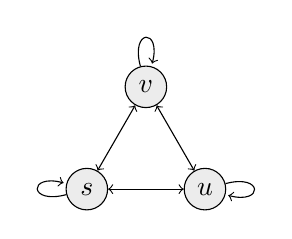
\begin{tikzpicture}
%[scale=1, transform shape]
  \foreach \pos/\name in {{(0,0)/s}, {+(0: 1.5)/u}, {+(60: 1.5)/v}}
        \node (\name) at \pos {$\name$};
   \foreach \from/\to in {s/u, u/v, v/s}
	\draw [<->] (\from) -- (\to);
   \path[]
	(s) edge[loop left] (s)
	(u) edge[loop right] (u)
	(v) edge[loop above] (v);
\end{tikzpicture}

&

$T = \{s, u, v\}$\newline
$d = 1$\newline
$|R| = 2$\

&

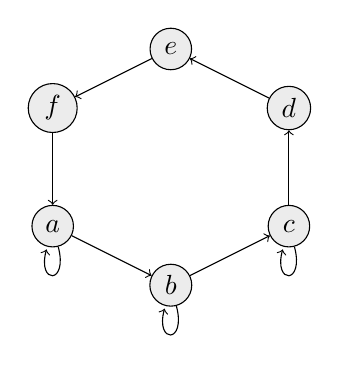
\begin{tikzpicture}
  \foreach \pos/\name in {{(0,0)/a}, {(1.5,-0.75)/b}, {(3,0)/c}, {(3,1.5)/d}, {(1.5,2.25)/e}, {(0,1.5)/f}}
        \node (\name) at \pos {$\name$};
   \foreach \from/\to in {a/b, b/c, c/d, d/e, e/f, f/a}
	\draw [->] (\from) -- (\to);

   \path[]
	(a) edge[loop below] (a)
	(b) edge[loop below] (b)
	(c) edge[loop below] (c);
	%(d) edge[loop above] (d)
	%(e) edge[loop above] (e)
	%(f) edge[loop above] (f);
\end{tikzpicture}

&

$T = \{a, b, c\}$\newline
$d = 3$\newline
$|R| = 2$\

\end{tabular}

\vspace{-5pt}
\caption{{Example settings of multi-robot patrolling games.}}
\label{fig:examples2}
\end{figure}

\begin{example}
\label{ex:joint}
Consider the MRPG from Fig.~\ref{fig:examples2} (left), which is played on a complete graph on 3 nodes.
All the nodes are targets with attack length 1 and the defender has two robots to patrol them.
The attack length 1 means that if the attacker attacks a node $t \in T$, he will be caught with probability equal to the probability that at least one robot will visit $t$ in the next step.
%That makes the objective of the defender to uniformly cover all the nodes in each step.

For a given defender's strategy $\sigma$, a history $h$ and a target $t$, let us denote by $p(t)$ the probability that $t$ will be visited in the next step, and by $p_2(t)$ the probability that both robots will visit $t$ in the next step.
As there are two robots, we have that $\sum_{t \in T}p(t) = 2 - \sum_{t \in T}p_2(t)$.
And as the value of the strategy is at most $\min_{t\in T} p(t)$, which is at most $\sum_{t \in T}p(t) / |T| = 2/3$, we have an upper bound $2/3$ on the value of the game.
This value can be achieved e.g. with a joint strategy $\sigma$ such that $\sigma(h)((s, u)) = \sigma(h)((s, v)) = \sigma(h)((u, v)) = 1/3$ for all $h \in \mathcal{H}_0$.

That said, every optimal strategy has to visit each target with probability $2/3$ in each step.
We show that this is impossible without coordination of movement between the robots.
In a disjointed strategy, each robot $r_i$ has its own strategy $\sigma_i$ depending only on its position and the resulting strategy $\sigma$ is a product of these strategies.
Let $h$ be an arbitrary history and $i \in \{1, 2\}$.
If $supp(\sigma_i(h)) = \{t\}$ for some $t \in T$, then robot $r_i$ visits $t$ with probability~$1$ and the other robot has to protect the remaining two targets.
However, that cannot be done better than with probability $1/2$.
Let us suppose, then, that $|supp(\sigma_i(h))| > 1$ for both $i$.
That means that there is a common target $t \in supp(\sigma_1(h)) \cup supp(\sigma_2(h))$, i.e. $p_2(t) > 0$.
From that we have $\sum_{t \in T}p(t) < 2$, which implies that $val(\sigma) < 2/3$.
Therefore, no optimal strategy for this game is a disjointed strategy.

%This cannot be done any other way than uniformly choosing a configuration with cover $\{s, u\}$, with cover $\{s, v\}$, or with cover $\{u, v\}$, each with probability $1/3$,
\end{example}

\begin{example}
\label{ex:initial2}
Consider the MRPG from Fig.~\ref{fig:examples2} (right).
It is not hard to find an optimal strategy with value $1$.
It suffices to initially put the two robots in diametrical nodes, e.g. $a$ and $d$, and then move them counterclockwise.

Now, let us assume that the initial configuration is a parameter of the game rather than determined by defender's strategy.
Consider the case when initial configuration is $(b, c)$.
The value of such a game is clearly $0$ as the shortest path from $c$ to $a$ is of length $4$.

This example demonstrates that even under some reasonable conditions ($(t, t) \in E$ for each $t \in T$, all robots start in mutually different targets), forcing an initial configuration might lower the value of the game.
Even forcing the set of edges $E$ to be a reflexive and symmetric relation over the set of nodes $U$ would not be enough---for a counterexample, consider a game played on a circle of 8 nodes with $T = U$, $d = 4$ and 2 robots starting next to each other.
\end{example}

\begin{example}
\label{ex:distribution}
For our last example, consider again the MRPG from Fig.~\ref{fig:examples2} (left).
From Example \ref{ex:joint}, we already know that the value of this game is $2/3$.
For now, let us assume that the attacker can attack before the robots are positioned in their $\sigma$-initial configuration.
Then the value of the game is clearly $0$ as the attacker can successfully attack the only target that is not covered by the $\sigma$-initial configuration (recall that $supp(\sigma(\epsilon))$ has to be a singleton).
Therefore, we do not allow the attacker to attack in step 0.
\end{example}

\section{TODO}

- co sa tyka 3.1, treba povedat, ze i tu existuje optimalna strategia - t.j. compact and continuous

\chapter{This is the end, my only friend, the end}

%centralne riadena strategia -> future work sa moze ubrat tymto (inym) smerom

%TODO list
%TODO spell checker
%TODO kedykolvek je nieco nove - preco je to nove/lepsie/hlbsi dokaz -> aby bolo vidiet, co som urobil

\def\us{\char`\_}

\bibliographystyle{plain}
\begin{thebibliography}{9}

\bibitem{perimeter} N. Agmon, S. Kraus, and G. A. Kaminka. Multi-Robot Perimeter Patrol in Adversarial Settings. In \emph{ICRA}, pages 2339�2345, 2008.

\bibitem{perimeter2} N. Agmon, V. Sadov, S. Kraus, and G. A. Kaminka. The Impact of Adversarial Knowledge on Adversarial Planning in Perimeter Patrol. In \emph{AAMAS}, pages 55-62, 2008.

\bibitem{perimeter3} N. Agmon, S. Kraus, G. A. Kaminka, and V. Sadov. Adversarial Uncertainty in Multi-Robot Patrol. In \emph{IJCAI}, pages 1811-1817, 2009.

\bibitem{arbitrary} N. Basilico, N. Gatti, and F. Amigoni. Leader-Follower Strategies for Robotic Patrolling in Environments with Arbitrary Topologies. In \emph{AAMAS}, pages 57-64, 2009.

\bibitem{powerlessIntruder} N. Basilico, N. Gatti, T. Rossi, S. Ceppi, and F. Amigoni. Extending Algorithms for Mobile Robot Patrolling in the Presence of Adversaries to More Realistic Settings. In \emph{WI-IAT}, pages 557-564, 2009.

\bibitem{multi-robot} N. Basilico, N. Gatti, and F. Villa. Asynchronous Multi-Robot Patrolling against Intrusion in Arbitrary Topologies. In \emph{AAAI}, pages 1224-1229, 2010.

\bibitem{movingTargets} B. Bo�ansk�, V. Lis�, M. Jakob, and M. P�chou�ek. Computing Time-Dependent Policies for Patrolling Games with Mobile Targets. In \emph{AAMAS}, pages 989-996, 2011.

\bibitem{line} F. Fang, A. X. Jiang, and M. Tambe. Optimal Patrol Strategy for Protecting Moving Targets with Multiple Mobile Resources. In \emph{AAMAS}, pages 957-964, 2013.

\bibitem{miso} M. Abaffy. Patrolling Games on Graphs [online]. 2013 [cit. 2014-05-10] ??? Diploma thesis. Masaryk University, Faculty of Informatics. Available at $<$http://is.muni.cz/th/321758/fi\texttt{\us}m/$>$.
%TODO

\bibitem{iti1} M. Abaffy, T. Br�zdil, V. �eh�k, B. Bo�ansk�, A. Ku�era, and J. Kr��l. Solving Adversarial Patrolling Games with Bounded Error. Online: ??? $<$http://goo.gl/ueKS79$>$
%TODO

\bibitem{iti2} T. Br�zdil, P. Hlin�n�, A. Ku�era, and V. �eh�k. Optimal Strategies in Adversarial Patrolling Games. Online: ???
%TODO

\bibitem{fudenberg} D. Fudenberg and J. Tirole. Game Theory. Cambridge, MA: \emph{MIT Press}, 1991.

\bibitem{polak} L. Pol�k. Teorie her [Lecture notes]. Masaryk University, Brno.

\bibitem{gameTheory} Game Theory [online]. [cit. 2014-05-23]. Available at
%\url{http://en.wikipedia.org/w/index.php?title=Game_theory&oldid=610438321}
% http://en.wikipedia.org/wiki/Game_theory
%$<$http://en.wikipedia.org/w/index.php?title=Game\texttt{\us}theory\&oldid=610438321$>$.
$<$http://en.wikipedia.org/wiki/Game\texttt{\us}theory$>$.

\bibitem{nash} J. F. Nash. Equilibrium Points in $n$-Person Games. In \emph{PNAS}, volume 36, pages 48�49, 1950.

\bibitem{convex} B. von Stengel and S. Zamir. Leadership Games with Convex Strategy Sets. \emph{Games and Economic Behavior}, volume 69, pages 446�457, 2010.

\bibitem{nashStack} J. Letchford and V. Conitzer. Computing Optimal Strategies to Commit to in Extensive-Form Games. In \emph{EC}, pages 83�92, 2010.

\bibitem{interchangability} Z. Yin, D. Korzhyk, C. Kiekintveld, V. Conitzer, and M. Tambe. Stackelberg vs. Nash in Security Games: Interchangeability, Equivalence, and Uniqueness. In \emph{AAMAS}, pages 1139�1146, 2010.

\bibitem{limited1} J. Pita, M. Jain, M. Tambe, F. Ord�$\rm{\tilde{n}}$ez, and S. Kraus. Robust Solutions to Stackelberg Games: Addressing Bounded Rationality and Limited Observations in Human Cognition. \emph{Artificial Intelligence}, volume 174, pages 1142-1171, 2010.

\bibitem{limited2} B. An, D. Kempe, C. Kiekintveld, E. Shieh, S. Singh, M. Tambe, and Y. Vorobeychik. Security Games with Limited Surveillance. In \emph{AAAI}, pages 1241�1248, 2012.

\bibitem{limited3} B. An, M. Brown, Y. Vorobeychik, and M. Tambe. Security Games with Surveillance Cost and Optimal Timing of Attack Execution. In \emph{AAMAS}, pages 223�230, 2013.

\bibitem{limited4} Y. Zhang and X. Luo. Security Games with Partial Surveillance. In \emph{AAMAS}, pages 1527-1528, 2014.

\bibitem{quantal} R. D. McKelvey and T. R. Palfrey. Quantal Response Equilibria for Normal Form Games. \emph{Games and Economic Behavior}, volume 10, pages 6�38, 1995.

\bibitem{armor} J. Pita, M. Jain, J. Marecki, F. Ord�$\rm{\tilde{n}}$ez, C. Portway, M. Tambe, C. Western, P. Paruchuri, and S. Kraus. Deployed ARMOR Protection: The Application of a Game Theoretic Model for Security at the Los Angeles International Airport. In \emph{AAMAS}, pages 125�132, 2008.

\bibitem{iris} J. Tsai, S. Rathi, C. Kiekintveld, F. Ord�$\rm{\tilde{n}}$ez, and M. Tambe. IRIS - A Tool for Strategic Security Allocation in Transportation Networks. In \emph{AAMAS}, pages 37-44, 2009.

\bibitem{guards} J. Pita, M. Tambe, C. Kiekintveld, S. Cullen, and E. Steigerwald. GUARDS - Game Theoretic Security Allocation on a National Scale. In \emph{AAMAS}, pages 37-44, 2011.

\bibitem{protect} E. Shieh, B. An, R. Yang, M. Tambe, C. Baldwin, J. DiRenzo, B. Maule, and G. Meyer. PROTECT: A Deployed Game Theoretic System to Protect the Ports of the United States. In \emph{AAMAS}, pages 13-20, 2012.

\bibitem{protect_coastguard} [cit. 2014-06-01] http://teamcore.usc.edu/projects/coastguard/
%TODO - maybe delete - no citation needed

\bibitem{trusts} Z. Yin, A. X. Jiang, M. P. Johnson, M. Tambe, C. Kiekintveld, K. Leyton-Brown, T. Sandholm, and J. P. Sullivan. TRUSTS: Scheduling Randomized Patrols for Fare Inspection in Transit Systems. In \emph{IAAI}, 2012.

\bibitem{trusts2} F. M. Delle Fave, M. Brown, C. Zhang, E. Shieh, A. X. Jiang, H. Rosoff, M. Tambe, and J. P. Sullivan. Security Games in the Field: an Initial Study on a Transit System. In \emph{AAMAS}, pages 1363-1364, 2014.

\bibitem{chung} K. L. Chung. Markov Chains with Stationary Transition Probabilities. Springer, 1967.

\bibitem{kucera} A. Ku�era. Turn-based stochastic games. In \emph{K. R. Apt and E. Gr�del. Lectures in Game Theory for Computer Scientists}, pages 146-184, 2011.

\bibitem{dfa} J. E. Hopcroft, R. Motwani, and J. D. Ullman. Introduction to Automata Theory, Languages, and Computation, 2nd edition. Addison Wesley, 2001. %page 46, 2001.

\end{thebibliography}

\end{document}